% !TeX program = pdflatex
% ============================================================
% OPERATING-VALUE SENSITIVITY — RESEARCH PAPER TEMPLATE
% Condensed scientific-paper format for a thesis-based valuation
% Target: <= 10 pages INCLUDING references.
% ============================================================

\documentclass[9pt,a4paper]{extarticle}

% ---------- Language & typography ----------
\usepackage[T1]{fontenc}
\usepackage[utf8]{inputenc}
\usepackage[english]{babel}
\usepackage{newtxtext,newtxmath}
\linespread{0.98}
\usepackage[protrusion=true,expansion=true]{microtype}
\usepackage[
  top=1.65cm,
  bottom=1.85cm,
  left=1.55cm,
  right=1.55cm,
  headheight=16pt,
  headsep=10pt,
  footskip=18pt
]{geometry}

% ---------- Core packages ----------
\usepackage{graphicx}
\usepackage{pdfpages}
\usepackage{xcolor}
\usepackage{booktabs}
\usepackage{array}
\usepackage{tabularx}
\usepackage{siunitx}
\usepackage{amsmath,mathtools,bm}
\usepackage{enumitem}
\usepackage{multicol}
\usepackage{caption}
\usepackage{subcaption}
\usepackage{float}
\usepackage{fancyhdr}
\usepackage{titlesec}
\usepackage[most]{tcolorbox}
\usepackage{natbib}
\usepackage{hyperref}
\usepackage[nameinlink,noabbrev]{cleveref}

% ---------- Palette ----------
% Academic first; club identity is intentionally subtle.
\definecolor{ink}{RGB}{29,29,31}
\definecolor{muted}{RGB}{92,92,98}
\definecolor{rulegray}{RGB}{180,180,184}
\definecolor{papergray}{RGB}{241,241,242}
\definecolor{brand}{RGB}{80,26,176}
\definecolor{accent}{RGB}{180,162,47}

% ---------- Metadata: edit these only ----------
\newcommand{\PaperType}{RESEARCH ARTICLE}
\newcommand{\PaperTitle}{Operating-Value Sensitivity for Barrick Mining}
\newcommand{\ShortTitle}{OPERATING-VALUE SENSITIVITY — BARRICK MINING CORPORATION}
\newcommand{\PaperSubtitle}{Option-implied gold and copper laws in a controlled operating experiment}
\newcommand{\PreparedDate}{07/09/2026}
\newcommand{\RevisedDate}{24/10/2026}
\newcommand{\PaperID}{Working Paper}
\newcommand{\JELCodes}{G12; G13; G31; C32; C53; C61; C63}

% Research teams. Keep team ownership visible rather than flattening the
% project into a single long author line.
\newcommand{\TeamOne}{Stefano Falcione; Marco Fracca}
\newcommand{\TeamTwo}{Filippo Triassi; Giorgio Zoccatelli}
\newcommand{\TeamThree}{Andrea Rostagno; Francesco Florio}
\newcommand{\TeamFour}{Giacomo Scali; Jacopo Foralosso}
\newcommand{\TeamFive}{Federico Vesco; Lorenzo Pietra; Bader Moussaif}
\newcommand{\TeamSix}{Davide Sisto; Matteo Armando}
\newcommand{\TeamSeven}{Davide D'Amico; Pietro Weisz}
\newcommand{\TeamEight}{Salvatore Gabriele Messina; Alessandro Coco}

% Numbers in the abstract and body come from sections/generated/results_20261024.tex,
% written by src/build_report_fragments.py from outputs/paper_audit_20261024.
% Generated by src/build_report_fragments.py from outputs/paper_audit_20261024.
% Do not edit by hand; rerun the generator after rebuilding the evidence.
\newcommand{\CalBSIVRMSE}{131.58}
\newcommand{\CalBSIVRMSELegacy}{97.21}
\newcommand{\CalHIVRMSE}{68.15}
\newcommand{\CalHIVRMSELegacy}{49.49}
\newcommand{\CalBIVRMSE}{65.24}
\newcommand{\CalBIVRMSELegacy}{49.41}
\newcommand{\CalWIVRMSE}{52.83}
\newcommand{\CalWIVRMSELegacy}{49.33}
\newcommand{\HawkesBranching}{0.825}
\newcommand{\HawkesBeta}{10.27}
\newcommand{\HawkesHalfLifeDays}{24.7}
\newcommand{\HawkesMeanIntensity}{1.65}
\newcommand{\BatesLambda}{1.72}
\newcommand{\HestonKappa}{2.93}
\newcommand{\FellerRelaxedLossRatio}{68}
\newcommand{\KappaFlatLow}{2}
\newcommand{\KappaFlatHigh}{4}
\newcommand{\CarryPriceRMSEZero}{0.49}
\newcommand{\CarryPriceRMSEFee}{0.75}
\newcommand{\FuturesYieldLow}{0.26}
\newcommand{\FuturesYieldHigh}{0.49}
\newcommand{\AmericanPremiumMax}{2.3e-10}
\newcommand{\ValBSMedian}{56.32}
\newcommand{\ValBSPTen}{4.31}
\newcommand{\ValBSPNinety}{160.19}
\newcommand{\ValBSMean}{71.94}
\newcommand{\ValBSNegative}{7.4}
\newcommand{\ValBSExplicit}{10.75}
\newcommand{\ValBSExplicitRiskFree}{11.81}
\newcommand{\ValHMedian}{57.62}
\newcommand{\ValHPTen}{0.13}
\newcommand{\ValHPNinety}{159.15}
\newcommand{\ValHMean}{71.63}
\newcommand{\ValHNegative}{9.9}
\newcommand{\ValHExplicit}{10.90}
\newcommand{\ValHExplicitRiskFree}{11.98}
\newcommand{\ValBMedian}{59.48}
\newcommand{\ValBPTen}{2.09}
\newcommand{\ValBPNinety}{156.74}
\newcommand{\ValBMean}{72.05}
\newcommand{\ValBNegative}{8.9}
\newcommand{\ValBExplicit}{11.08}
\newcommand{\ValBExplicitRiskFree}{12.19}
\newcommand{\ValWMedian}{57.26}
\newcommand{\ValWPTen}{1.26}
\newcommand{\ValWPNinety}{155.88}
\newcommand{\ValWMean}{73.11}
\newcommand{\ValWNegative}{9.3}
\newcommand{\ValWExplicit}{10.90}
\newcommand{\ValWExplicitRiskFree}{11.97}
\newcommand{\BarBS}{37.87}
\newcommand{\BarH}{38.75}
\newcommand{\BarB}{40.00}
\newcommand{\BarW}{38.51}
\newcommand{\ValMedianLow}{56.32}
\newcommand{\ValMedianHigh}{59.48}
\newcommand{\ValExplicitLow}{10.75}
\newcommand{\ValExplicitHigh}{11.08}
\newcommand{\ValPNinetyLow}{155.88}
\newcommand{\ValPNinetyHigh}{160.19}
\newcommand{\TerminalShare}{83}
\newcommand{\NumericalMedianLow}{56.24}
\newcommand{\NumericalMedianHigh}{59.99}
\newcommand{\NumericalHawkesLow}{56.26}
\newcommand{\NumericalHawkesHigh}{58.42}
\newcommand{\AttLegacyBS}{60.10}
\newcommand{\AttLegacyH}{59.77}
\newcommand{\AttLegacyB}{59.12}
\newcommand{\AttLegacyW}{59.82}
\newcommand{\AttClockBS}{57.81}
\newcommand{\AttClockH}{58.65}
\newcommand{\AttClockB}{59.34}
\newcommand{\AttClockW}{58.49}
\newcommand{\AttAnchorBS}{57.11}
\newcommand{\AttAnchorH}{57.95}
\newcommand{\AttAnchorB}{58.59}
\newcommand{\AttAnchorW}{57.74}
\newcommand{\AttCarryBS}{56.32}
\newcommand{\AttCarryH}{57.62}
\newcommand{\AttCarryB}{59.48}
\newcommand{\AttCarryW}{57.26}
\newcommand{\CuBSGold}{12.060}
\newcommand{\CuBSCombined}{14.368}
\newcommand{\CuBSDelta}{2.308}
\newcommand{\CuBSSE}{17.9}
\newcommand{\CuHGold}{11.981}
\newcommand{\CuHCombined}{14.285}
\newcommand{\CuHDelta}{2.304}
\newcommand{\CuHSE}{28.5}
\newcommand{\CuBGold}{12.062}
\newcommand{\CuBCombined}{14.379}
\newcommand{\CuBDelta}{2.317}
\newcommand{\CuBSE}{31.5}
\newcommand{\CuWGold}{12.154}
\newcommand{\CuWCombined}{14.484}
\newcommand{\CuWDelta}{2.330}
\newcommand{\CuWSE}{28.1}
\newcommand{\CuDeltaLow}{2.30}
\newcommand{\CuDeltaHigh}{2.33}
\newcommand{\TerminalWACC}{8.445}
\newcommand{\TerminalMultiple}{13.14}
\newcommand{\WACCClippedShare}{0.00}
\newcommand{\HorizonYears}{4.33}
\newcommand{\StubDays}{28}
\newcommand{\CovBSNinetyFive}{27/29}
\newcommand{\CovBSNinetyFiveP}{0.655}
\newcommand{\CovBSEighty}{21/29}
\newcommand{\CovBSEightyP}{0.350}
\newcommand{\CovHNinetyFive}{27/29}
\newcommand{\CovHNinetyFiveP}{0.655}
\newcommand{\CovHEighty}{20/29}
\newcommand{\CovHEightyP}{0.160}
\newcommand{\CovBNinetyFive}{25/29}
\newcommand{\CovBNinetyFiveP}{0.055}
\newcommand{\CovBEighty}{17/29}
\newcommand{\CovBEightyP}{0.008}
\newcommand{\CovWNinetyFive}{25/29}
\newcommand{\CovWNinetyFiveP}{0.055}
\newcommand{\CovWEighty}{16/29}
\newcommand{\CovWEightyP}{0.004}
\newcommand{\OosBSRMSE}{163.35}
\newcommand{\OosBSRMean}{-2.33}
\newcommand{\OosBSRPersistence}{-423.92}
\newcommand{\OosBSBeatsPersistence}{0}
\newcommand{\OosBSDMPersistenceP}{0.000}
\newcommand{\OosHRMSE}{89.62}
\newcommand{\OosHRMean}{69.17}
\newcommand{\OosHRPersistence}{-59.00}
\newcommand{\OosHBeatsPersistence}{4}
\newcommand{\OosHDMPersistenceP}{0.001}
\newcommand{\OosBRMSE}{68.39}
\newcommand{\OosBRMean}{80.62}
\newcommand{\OosBRPersistence}{-17.47}
\newcommand{\OosBBeatsPersistence}{14}
\newcommand{\OosBDMPersistenceP}{0.088}
\newcommand{\OosWRMSE}{64.16}
\newcommand{\OosWRMean}{83.03}
\newcommand{\OosWRPersistence}{-1.84}
\newcommand{\OosWBeatsPersistence}{13}
\newcommand{\OosWDMPersistenceP}{0.772}
\newcommand{\OosDMHawkesVsBSP}{0.000}
\newcommand{\OosDMHawkesVsHP}{0.000}
\newcommand{\OosDMHawkesVsBP}{0.165}
\newcommand{\OosDates}{30}
\newcommand{\OosObservations}{4,667}
\newcommand{\OosPersistenceObservations}{4,026}
\newcommand{\OosPersistenceRMSE}{58.31}
\newcommand{\FigOosRmse}{../img/publication/7d3e5597f15ab728_oos_rmse.png}
\newcommand{\FigOosRsquared}{../img/publication/19d304216f437e9e_oos_r2.png}
\newcommand{\FigFigValPrimary}{../img/publication/0e6f7e2f5b6abc45_fig_val_primary.png}
\newcommand{\FigFigValMulti}{../img/publication/893e0badbf0a67cf_fig_val_multi.png}
\newcommand{\FigFigTerminalShare}{../img/publication/36af633f72f0ca22_fig_terminal_share.png}
\newcommand{\FigFigCorrectionAttribution}{../img/publication/6d67719615b71840_fig_correction_attribution.png}
\newcommand{\FigBlackScholesResidualHeatmap}{../img/publication/612c9067fff153cc_black_scholes_residual_heatmap.png}
\newcommand{\FigHestonResidualHeatmap}{../img/publication/ba2dd686e32e5e10_heston_residual_heatmap.png}
\newcommand{\FigBatesResidualHeatmap}{../img/publication/917f624afe7e339f_bates_residual_heatmap.png}
\newcommand{\FigBatesHawkesResidualHeatmap}{../img/publication/38343b91b0c0ad53_bates_hawkes_residual_heatmap.png}
\newcommand{\FigArfimaFdSilver}{../img/publication/a47ac9bb3870cd03_arfima_fd_silver.png}
\newcommand{\GphGoldAbs}{0.452}
\newcommand{\GphSilverAbs}{0.743}

\newcommand{\PaperAbstract}{%
We ask how much the choice of gold-price model matters for a discounted operating-margin proxy of Barrick when production, costs and discount-rate shocks are held fixed. Black--Scholes, Heston, Bates and Bates--Hawkes are calibrated to 64 GLD calls of 2 September 2026, with the trust's 0.40\% sponsor fee treated as carry, and drive daily gold paths from the spot price at the valuation time. Only cash flows after the valuation date are counted. Across 8,192 paths the median proxy lies between USD~\ValMedianLow{} and \ValMedianHigh{}~bn for all four models, a spread no larger than the numerical sensitivity of a single model (USD~\NumericalMedianLow--\NumericalMedianHigh~bn across path counts and seeds). The terminal value accounts for about \TerminalShare\% of the mean. In 30 rolling repricing tests Bates--Hawkes has the lowest error, but no model beats the persistence of the implied-volatility surface. Three producing copper mines add about USD~\CuDeltaLow--\CuDeltaHigh~bn of explicit flows to 2030. The proxy has no equity bridge; it is a controlled research sensitivity, not a fair value, target price or investment recommendation.%
}
% ---------- Hyperlinks ----------
\hypersetup{
  colorlinks=true,
  hypertexnames=false,
  linkcolor=brand,
  citecolor=brand,
  urlcolor=brand,
  pdftitle={\PaperTitle},
  pdfauthor={Starting Finance Club PoliTo Research}
}

% ---------- Global paragraph settings ----------
\setlength{\parindent}{1em}
\setlength{\parskip}{0pt}
\setlength{\columnsep}{0.62cm}
\setlength{\columnseprule}{0pt}
\raggedbottom

% ---------- Section style ----------
\titleformat{\section}
  {\normalfont\bfseries\fontsize{9.4}{10.8}\selectfont\color{ink}\raggedright\MakeUppercase}
  {\thesection}{0.65em}{}
\titlespacing*{\section}{0pt}{9pt}{3pt}

\titleformat{\subsection}
  {\normalfont\bfseries\fontsize{9.1}{10.5}\selectfont\color{ink}\raggedright}
  {\thesubsection}{0.55em}{}
\titlespacing*{\subsection}{0pt}{6pt}{2pt}

\titleformat{\subsubsection}
  {\normalfont\itshape\fontsize{8.9}{10.3}\selectfont\color{ink}\raggedright}
  {\thesubsubsection}{0.5em}{}
\titlespacing*{\subsubsection}{0pt}{5pt}{1.5pt}

% ---------- Header / footer ----------
\pagestyle{fancy}
\fancyhf{}
\fancyhead[L]{\fontsize{7.3}{8.5}\selectfont\color{muted}\ShortTitle}
\fancyhead[R]{\fontsize{7.3}{8.5}\selectfont\color{muted}STARTING FINANCE CLUB POLITO — RESEARCH}
\fancyfoot[C]{\fontsize{7.1}{8}\selectfont\color{muted}\thepage}
\renewcommand{\headrulewidth}{0.35pt}
\renewcommand{\footrulewidth}{0pt}

\fancypagestyle{firstpage}{%
  \fancyhf{}
  \fancyfoot[C]{\fontsize{7.1}{8}\selectfont\color{muted}\thepage}
  \renewcommand{\headrulewidth}{0pt}
  \renewcommand{\footrulewidth}{0pt}
}

% ---------- Captions ----------
\captionsetup{
  hypcap=false,
  font=footnotesize,
  labelfont=bf,
  labelsep=period,
  justification=raggedright,
  singlelinecheck=false,
  skip=2pt
}

% ---------- Lists ----------
\setlist[itemize]{leftmargin=1.2em,itemsep=1pt,topsep=3pt,parsep=0pt}
\setlist[enumerate]{leftmargin=1.3em,itemsep=1pt,topsep=3pt,parsep=0pt}

% ---------- Tables ----------
\sisetup{
  detect-all,
  group-separator={,},
  group-minimum-digits=4,
  table-number-alignment=center
}
\renewcommand{\arraystretch}{1.08}

% ---------- Reusable scientific-paper boxes ----------
\newtcolorbox{findingbox}[1][Key finding]{
  colback=papergray,
  colframe=rulegray,
  boxrule=0.45pt,
  arc=0pt,
  left=5pt,right=5pt,top=4pt,bottom=4pt,
  before skip=5pt,after skip=5pt,
  fonttitle=\bfseries\fontsize{8.4}{9.5}\selectfont,
  title=#1
}

\newtcolorbox{methodbox}[1][Methodological note]{
  colback=brand!3,
  colframe=brand!35,
  boxrule=0.45pt,
  arc=0pt,
  left=5pt,right=5pt,top=4pt,bottom=4pt,
  before skip=5pt,after skip=5pt,
  fonttitle=\bfseries\fontsize{8.4}{9.5}\selectfont,
  title=#1
}

% ---------- Compact equation helper ----------
\newcommand{\E}{\mathbb{E}}
\newcommand{\Var}{\mathrm{Var}}
\newcommand{\Cov}{\mathrm{Cov}}
\newcommand{\Prob}{\mathbb{P}}
\newcommand{\dd}{\,\mathrm{d}}

% ---------- Title-page helpers ----------
\newcommand{\topmetadata}{%
  \begingroup
  \setlength{\parindent}{0pt}%
  \noindent
  \begin{minipage}[c]{0.75\textwidth}
    \fontsize{7.0}{8.4}\selectfont\color{muted}\PreparedDate\enspace | Revised \RevisedDate
  \end{minipage}%
  \hfill
  \begin{minipage}[c]{0.19\textwidth}\raggedleft
    
\includegraphics[height=24pt]{../img/publication/572456d904007768_Logo_SFClub_Polito.png}
  \end{minipage}\par
  \vspace{2pt}
  {\color{rulegray}\rule{\textwidth}{0.45pt}}\par
  \vspace{7pt}
  {\fontsize{7.5}{9}\selectfont\bfseries\textls[130]{\PaperType}\par}
  \vspace{12pt}
  \endgroup
}


% ---------- Research-team author grid ----------
\newcommand{\teamrow}[4]{%
  \textbf{Team #1}\enspace #2 & \textbf{Team #3}\enspace #4 \\
}

\newcommand{\authorgrid}{%
\begingroup
\setlength{\tabcolsep}{7pt}%
\renewcommand{\arraystretch}{1.23}%
\noindent\begin{tabularx}{\textwidth}{@{}>{\raggedright\arraybackslash}X>{\raggedright\arraybackslash}X@{}}
\teamrow{1}{\TeamOne}{2}{\TeamTwo}
\teamrow{3}{\TeamThree}{4}{\TeamFour}
\teamrow{5}{\TeamFive}{6}{\TeamSix}
\teamrow{7}{\TeamSeven}{8}{\TeamEight}
\end{tabularx}
\endgroup
}

% ---------- Abstract panel ----------
\newcommand{\abstractpanel}{%
\begin{tcolorbox}[
  colback=papergray,
  colframe=papergray,
  boxrule=0pt,
  arc=0pt,
  left=7pt,right=7pt,top=6pt,bottom=6pt,
  width=\linewidth
]
{\bfseries\fontsize{8.5}{10}\selectfont Abstract}\par\vspace{2pt}
{\fontsize{8.05}{9.75}\selectfont
\PaperAbstract\par}

\end{tcolorbox}
}

% ============================================================
% DOCUMENT
% ============================================================
\begin{document}
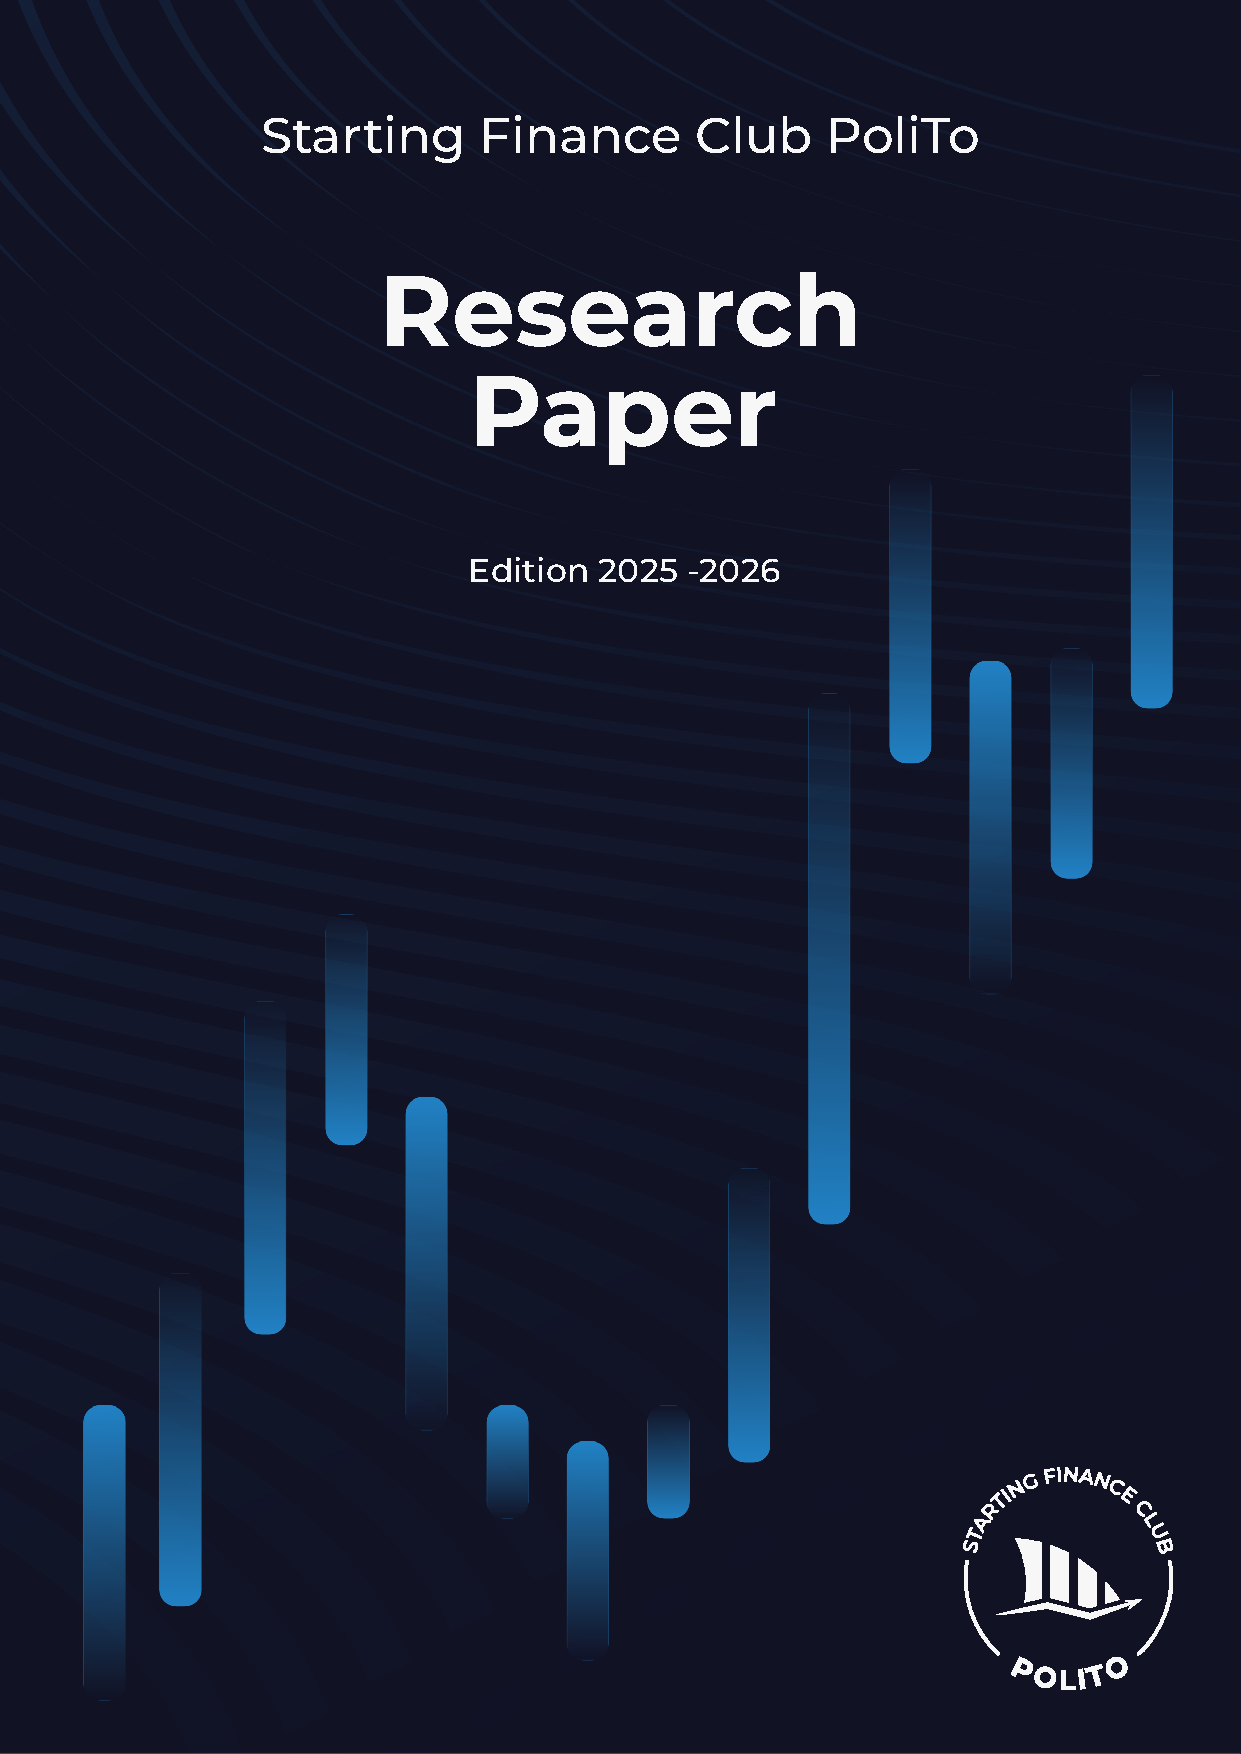
\includepdf[pages=1]{Copertina_research.pdf}
\setcounter{page}{1}
\thispagestyle{firstpage}
\fontsize{8.85}{10.55}\selectfont

% ----- Journal-like first-page masthead -----
\topmetadata

% ----- Title -----
{\noindent\fontsize{18.5}{21}\selectfont\bfseries\color{ink}\PaperTitle\par}
\vspace{3pt}
{\noindent\fontsize{9.3}{11}\selectfont\itshape\color{muted}\PaperSubtitle\par}
\vspace{11pt}

% ----- Authors: research teams paired across two columns -----
{\fontsize{7.85}{9.4}\selectfont\authorgrid}
\vspace{8pt}

% ----- Research affiliation + abstract layout inspired by academic journals -----
\noindent
\begin{minipage}[t]{0.28\textwidth}
  \vspace{0pt}
  {\fontsize{7.2}{8.85}\selectfont
  \textbf{Contacts --}\par
  \textbf{Starting Finance Club PoliTO}\par\vspace{3pt}
  \href{https://www.linkedin.com/company/startingfinance-club-polito}{\raisebox{-1pt}{
\includegraphics[height=8pt]{../img/publication/19547bce5dddbce5_contact_linkedin.png}}\,LinkedIn}\enspace
  \href{https://sfclubpolito.it/}{\raisebox{-1pt}{
\includegraphics[height=8pt]{../img/publication/385027198bc15712_contact_website.png}}\,Website}\par
  \href{https://github.com/StartingFinanceClubPoliTo/Research}{\raisebox{-1pt}{
\includegraphics[height=8pt]{../img/publication/79d19491a73dad7e_contact_github.png}}\,GitHub}\enspace
  \href{https://www.instagram.com/sfclubpolito}{\raisebox{-1pt}{
\includegraphics[height=8pt]{../img/publication/31b19f2ba436aac3_contact_instagram.png}}\,Instagram}\par
  \href{mailto:startingfinanceclub@studenti.polito.it}{\raisebox{-1pt}{
\includegraphics[height=8pt]{../img/publication/8fedf2bb8bed3ca1_contact_email.png}}\,Institutional email}\par\vspace{3pt}
  \textbf{JEL classification}\par
  \JELCodes\par
  \vspace{3pt}
  \textbf{Discoveries}\par\vspace{2pt}
  Median proxy under each gold law,\par
  common operating contract.\par\vspace{3pt}
  {\setlength{\tabcolsep}{0pt}\renewcommand{\arraystretch}{1.18}%
  \begin{tabular}{@{}p{59pt}p{47pt}r@{}}
  Black--Scholes & \textcolor{brand!55}{\rule{\BarBS pt}{4pt}} & \ValBSMedian\\
  Heston & \textcolor{brand!65}{\rule{\BarH pt}{4pt}} & \ValHMedian\\
  Bates--Poisson & \textcolor{brand!75}{\rule{\BarB pt}{4pt}} & \ValBMedian\\
  Bates--Hawkes & \textcolor{brand}{\rule{\BarW pt}{4pt}} & \ValWMedian
  \end{tabular}}\par\vspace{3pt}
  USD billion; signed terminal value.\par
  Monte Carlo range of one model:\par
  \NumericalMedianLow--\NumericalMedianHigh. Not company value.\par
  }
\end{minipage}%
\hfill
\begin{minipage}[t]{0.69\textwidth}
  \vspace{0pt}
  \abstractpanel
\end{minipage}

\vspace{9pt}

% ============================================================
% BODY — CONTINUOUS TWO-COLUMN FLOW
% Figures stay within the continuous two-column flow.
% ============================================================
\begin{multicols}{2}
\raggedcolumns
\section*{Research programme and collaboration}
This paper grew out of an eight-team project involving 17 students with complementary backgrounds in mathematics, data science, engineering, economics and finance. The size of the author group reflects a division of research responsibilities and a shared learning process: Teams 1--3 developed the mathematical, econometric and simulation foundations; Teams 4--5 built the operating and corporate-valuation layers; and Teams 6--8 studied gold-price dynamics, market evidence and option-implied calibration.

The extended \href{https://raw.githubusercontent.com/StartingFinanceClubPoliTo/Research/main/Barrick-Gold/Barrick\%20Mining\%20UNIFICATO/thesis/Articolo.pdf}{technical report} records definitions, derivations and implementation choices to establish a common technical language across these backgrounds. Teams worked on dedicated modules, then compared assumptions, revised their contributions and reconciled dates, units and interfaces before integration. The present paper condenses this work into a single auditable experiment. Together with the reproducible code, it demonstrates the group's existing research practice and provides a basis for developing a sustained student-led quantitative research team with academic guidance.

\section{Introduction}
A gold producer's value depends on the distribution of future commodity prices as well as its operating and financing assumptions. A single price path can hide this source of model risk. We ask how an unconstrained Barrick operating-proxy distribution changes when progressively richer gold-price processes are substituted within a common operating scenario and discounted-margin contract.

We compare Black--Scholes, Heston, Bates--Poisson and Full Bates--Hawkes calibrated to GLD options. Current-surface diagnostics and rolling out-of-sample tests distinguish fit from predictive performance; shared production, costs and WACC shocks isolate the effect of the gold engine. The contribution is this controlled comparison and its auditable integration, rather than a claim that any model provides an unconditional fair value.

\columnbreak
\section{Data and Valuation Setup}

\subsection{Controlled layer separation}
The integrated experiment is organized as a controlled handoff across three modules. Team 8 governs only the gold-price process; Team 4 supplies the operating forecasts; and Team 5 maps those inputs through a common tax, WACC and terminal-value contract without a reconciled equity bridge. In the four-model comparison only the gold engine changes: the same Team 4 production and unit-cost forecasts, the same Team 5 corporate rules and the same WACC shocks are reused across runs.

\subsection{Valuation clock}
The valuation time is the 2 September 2026 close (20:00~UTC). Only flows after it are valued. Barrick's Q1--Q2 2026 actuals have already been realised and are excluded; they are used only to check levels. The quarter that contains the valuation date contributes its remaining \StubDays{} of 92 days, under the stated assumption that production and unit cost are uniform within the quarter. Eighteen quarters follow, to 31 December 2030 (\HorizonYears{} years). Revenue in each quarter uses the average simulated daily gold price over its remaining interval, and each flow is discounted from the midpoint of that interval.

\subsection{Calibration snapshot and carry}
The calibration uses the 2 September 2026 GLD call surface acquired through the IB API. After the common DTE $\geq75$ and numerical filters, the dense surface contains 605 eligible observations across 12 expiries and 146 strikes, with 79--653 days to expiry. The $8\times8$ Chebyshev--Chebyshev sample contains 64 distinct actual contracts spanning eight expiries and 20 strikes. The rate input is a same-date NSS fit to 14 U.S. Treasury tenors \citep{nss1994,treasury2026}, with a 2.0608~bp RMSE against the continuously compounded par-yield proxy; it is not a bootstrapped zero curve.

GLD's sponsor fee of 0.40\% a year reduces the gold backing of each share, so the GLD forward is $S e^{(r-q)T}$ with $q=0.40\%$ even though no cash is distributed \citep{spdr2025}. Two independent observations support this value: the GLD/gold log-ratio trend of $-0.396\%$ a year over 2022--2026, and COMEX gold futures, whose carry against the synchronous spot implies a GLD yield of \FuturesYieldLow--\FuturesYieldHigh\% at 0.5--0.8 years. The carry is applied exactly through $C(S,K;q)=e^{-qT}C(S,Ke^{qT};0)$.

The gold scenarios start from the XAUUSD spot of USD~4,391.32/oz at the valuation time, synchronous with the GLD close. The earlier draft started from Barrick's Q2 average realised price of USD~4,417/oz, which predates the valuation by two months.

\subsection{Probability measure}
Option parameters are estimated under $\mathbb Q$. The scenario drift is the integral-preserving forward curve of the Treasury fit. Read as a physical expectation, this assumes no gold risk premium, which is a common assumption for an asset with near-zero market beta but is not estimated here. The option-implied volatility shape is carried over as a conditional assumption; it is not a validated physical law. Expected flows are then discounted at WACC, as in an ordinary DCF. For comparison, Section~\ref{sec:results} also reports the explicit flows discounted at the risk-free curve. A full $\mathbb Q\rightarrow\mathbb P$ specification would need price, variance and jump risk premia (Section~\ref{sec:paper-physical-measure}).

\begin{table}[H]
\centering
\caption{Contract held fixed across gold engines.}
\label{tab:frozen_contract}
\begin{tabularx}{\columnwidth}{@{}>{\bfseries}p{0.25\columnwidth}X@{}}
\toprule
Block & Current experiment \\
\midrule
Gold layer & Black--Scholes/GBM, Heston, Bates--Poisson and Full Bates--Hawkes calibrated by Team 8 under $\mathbb Q$ with $q=0.40\%$. \\
Operations & Team 4 production and unit-cost forecasts from 2026Q3 (stub) to 2030Q4; actuals excluded. \\
Corporate mapping & Team 5 tax, growth--ROIC--reinvestment schedule, stochastic WACC and explicit terminal convention; no equity bridge. \\
Simulation & 8,192 paths, daily steps, one common WACC shock array. \\
\bottomrule
\end{tabularx}
\end{table}

\subsection{Option exercise convention}
GLD contracts are American-style \citep{cboe2026}. With $q=0.40\%$ below the Treasury rate, early exercise of a call is not optimal in the frictionless model. An 800-step CRR check on all 64 contracts gives a maximum American--European premium of USD~\AmericanPremiumMax; this tests the convention, not market frictions.

\subsection{Operating-model status}
Team 4's original operating study is richer than the object passed downstream. Cost of Sales is forecast from a log-space master chain; production is constructed bottom-up from ore processed, average grade and recovery. The valuation uses the resulting point forecasts, so mine-level operating uncertainty is not propagated jointly with gold-price uncertainty. Team 4's legacy price simulation and illustrative EBITDA/valuation output are excluded.

\subsection{Gold perimeter and reporting basis}
The Team 4 subset comprises Bulyanhulu, Carlin, Cortez, Kibali, Loulo--Gounkoto, North Mara, Pueblo Viejo and Turquoise Ridge. Its quarterly estimation window is 2019Q1--2025Q4, with North Mara beginning in 2019Q4. The operating quantities are already attributable: Nevada Gold Mines is 61.5\%, Pueblo Viejo 60\%, Kibali 45\%, Loulo--Gounkoto 80\%, and the Tanzanian mines 84\%. Kibali is equity-accounted, whereas the other interests are consolidated with partners' non-controlling interests \citep{barrickar2025}. Those partners must not be deducted again from attributable flows. Tanzania's contractual economic-benefit sharing still requires a separate cash-flow reconciliation.

The forecast covers the eight-mine subset, which produced 622 and 711~koz in Q1--Q2 2026 against company-wide totals of 719 and 796~koz. The proxy therefore omits the remaining gold mines. Cost of Sales includes depreciation and price-sensitive royalties; multiplying its sold-ounce cost by production gives a component-margin proxy, not EBITDA or reconciled EBIT. Loulo--Gounkoto's 2025Q4 accounting uplift also makes its cost anchor a normalization issue. Ownership, the North America IPO, cash and debt, share count and reserves must be fixed at the valuation date before any per-share result can be reported.

\section{Methodology}

\subsection{Gold-price engines}
The four Team 8 specifications relax one restriction at a time. Under $\mathbb Q$, Black--Scholes/GBM uses constant volatility,
\begin{equation}
\frac{\dd S_t}{S_t}=(r_t-q_t)\dd t+\sigma\dd W_t.
\label{eq:gbm}
\end{equation}
GBM is the constant-volatility benchmark.
Heston introduces mean-reverting stochastic variance \citep{heston1993},
\begin{align}
\frac{\dd S_t}{S_t}&=(r_t-q_t)\dd t+\sqrt{v_t}\dd W_t^{S},\\
\dd v_t&=\kappa(\theta-v_t)\dd t+\xi\sqrt{v_t}\dd W_t^{v},
\qquad \dd W_t^S\dd W_t^v=\rho\dd t.
\label{eq:heston}
\end{align}
Bates adds compensated compound-Poisson jumps \citep{bates1996},
\begin{equation}
\frac{\dd S_t}{S_{t^-}}=(r_t-q_t-\lambda k)\dd t+\sqrt{v_t}\dd W_t^S+(e^J-1)\dd N_t,
\label{eq:bates}
\end{equation}
where $k=\E^{\mathbb Q}[e^J-1]$.

\subsection{Full Bates--Hawkes: implemented affine engine}
The full engine preserves Heston variance but replaces the constant Poisson arrival rate with an exponential Hawkes state \citep{hawkes1971}:
\begin{align}
\frac{\dd S_t}{S_{t^-}}&=(r_t-q_t-\lambda_t k)\dd t+\sqrt{v_t}\dd W_t^S+(e^J-1)\dd N_t,\\
\dd v_t&=\kappa(\theta_v-v_t)\dd t+\xi\sqrt{v_t}\dd W_t^v,\\
\dd\lambda_t&=\beta(\bar\lambda-\lambda_t)\dd t+\alpha\dd N_t,
\qquad n=\alpha/\beta<1.
\label{eq:full_bh_sde}
\end{align}
Under the implemented exponential-kernel specification, pricing exploits the affine Markov structure rather than a standalone finite-difference PIDE. Writing $X_t=\log S_t$, the characteristic function factorizes into Heston diffusion and Hawkes jump blocks,
\begin{equation}
\phi_{X_T}(u)=\phi_{\mathrm{diff}}(u)\exp\!\left(A(u,T)+B(u,T)\lambda_0\right),
\label{eq:bh_cf}
\end{equation}
with the jump block determined by the Riccati system
\begin{align}
\frac{\dd B}{\dd\tau}&=\psi_J(u)e^{\alpha B}-\beta B-iuk-1,\\
\frac{\dd A}{\dd\tau}&=\beta\bar\lambda B,
\qquad A(0)=B(0)=0,
\label{eq:bh_riccati}
\end{align}
where $\psi_J(u)=\exp(iu\mu_J-\tfrac12\sigma_J^2u^2)$. European call prices use Fourier-COS inversion \citep{cos2008}, with independent diffusion and jump drivers. The identities $\phi(0)=1$, the martingale condition at $u=-i$, and the limit $\alpha\to0$, $\lambda_0=\bar\lambda$, back to Bates are used as implementation checks.

\begin{methodbox}[Model-role constraint]
These processes govern commodity prices only. The copper extension uses forward-price analogues; neither price layer generates Barrick production or costs.
\end{methodbox}

\subsection{Option-surface calibration and predictive test}
Every model is fitted to the same structured GLD surface by minimizing a vega-scaled price loss,
\begin{equation}
F(\theta)=\frac{1}{N}\sum_{i=1}^{N}
\left[\frac{C_i^{model}(\theta)-C_i^{mkt}}
{\max(\mathrm{Vega}_i,\varepsilon)}\right]^2,
\label{eq:calibration_loss}
\end{equation}
with Vega per unit decimal volatility and $\varepsilon=10^{-4}$. This is price-based MSE; exact IV RMSE uses inversion, a square root and $10^4$ scaling. Nested starts are retained during SLSQP refinement. A Feller strict-positivity constraint is imposed by choice; Hawkes stability requires $n<1$.

Calibration fit and forecasting are evaluated separately. A date is admitted to the rolling test only when at least 64 eligible observations and three expiries survive the common filters. Each CC64 origin is scored on the next dense date. With $n_t$ common targets on date $t$, equal-date performance is
\begin{equation}
R^2_{OOS,m\mid b}=1-\frac{\sum_t n_t^{-1}\sum_j e_{m,t,j}^2}{\sum_t n_t^{-1}\sum_j e_{b,t,j}^2},
\label{eq:oos_r2}
\end{equation}
against both the origin cross-sectional mean IV and an origin observed-IV surface interpolated in maturity and log-moneyness inside its convex hull. The target spot and rate curve enter only as scoring-date conditioning variables. This design prevents the lowest in-sample IV error from being interpreted automatically as predictive dominance.

% Expansion p2 - 2026-09-06
Origin parameters are frozen before next-date scoring; target quotes do not select them. Conditioning on target spot and rates makes this a repricing test, not a joint ex ante forecast. Persistence is evaluated only on its interpolation support; unmatched observations are not zero losses.

\subsection{From pricing measure to physical revenues}
\label{sec:paper-physical-measure}
Option coefficients under $\mathbb Q$ do not identify physical commodity
returns. All four families can be estimated under $\mathbb P$, but their
cross-measure link requires underlying history and identified risk premia
\citep{pan2002}. With
$\dd W^Q=\dd W^P+\eta\sqrt v\dd t$, the restricted variance map is
$\kappa_P=\kappa_Q-\xi\eta_v$ and
$\kappa_P\theta_P=\kappa_Q\theta_Q$.
A positive intensity scaling $c_I$ and normal mark tilt give
$\lambda_P=c_I\lambda_Q$ and
$\mu_{J,P}=\mu_{J,Q}+b_J\sigma_J^2$. Thus physical expected price return is
\begin{equation}
\mu_t^P=a_t^Q+\eta_Sv_t+
\lambda_t^Q(c_Ik_P-k_Q),
\label{eq:paper-physical-drift}
\end{equation}
where $a_t^Q$ is pricing carry and $k_M=\mathbb E^M[e^J-1]$.
Hawkes baseline, initial intensity and excitation scale by $c_I$, while
decay is unchanged; physical branching must stay below one. Algebraic
closure does not identify premia. For the restricted CIR and unmarked linear
Hawkes family, a stopped-density entropy bound establishes equivalence on
finite horizons; its full assumptions and derivation are in the unified
study \citep{schonbucher2001,sokol-hansen2015}. Empirical estimation and
predictive validation remain separate. In
particular, copper Bates has zero fitted $Q$ jump intensity: an equivalent
change cannot create physical jumps without a new joint specification.

The 6 October diagnostic, still cut off at 2 September, adds 1,253 GLD
regular-session prices and 1,003 synchronous GLD--gold observations,
including early closes. Seven copper deliveries provide 408 accepted
origin-selected, same-delivery returns; four requested earlier deliveries
were unavailable. This avoids artificial rollover jumps but does not
identify copper spot carry or realised selling prices. The approximately
100-contract option budget is separate from the daily time-series sample.

A training-only GLD GBM with an origin-fitted gold basis produces quarterly
gold-price RMSE of USD~417.19/oz over 689 overlapping targets, versus
USD~428.52/oz for a no-change mean. Its nominal 95\% coverage is only
89.6\%; direct gold GBM has better absolute error and log score. This is a
physical historical benchmark, not a joint option/history fit. Preliminary
fixed-current-$Q$ Heston, Bates and Hawkes premium estimates remain sensitive
to particle and time-step resolution and are not admitted to valuation.

Option repricing OOS, physical commodity OOS and Barrick operating OOS are
distinct tests. Current pricing coefficients cannot be used at earlier
physical forecast origins. The intended DCF requires $\mathbb P$ realised
selling prices. Thirty recovered historical surfaces, each with 64 contracts,
permit new dated calibrations. A conditional two-stage estimator may fit
$\mathbb Q$ options and then physical premia using origin-available returns;
it is not joint maximum likelihood and must address uncertainty from both
stages. Forward paths share the option-estimated initial state across measures.
All four physical models now have 29 common next-session targets.
After origin-only gold conversion, RMSE is USD~66.35/oz for GBM, 66.77
for Heston, 66.84 for Bates and 65.81 for Bates--Hawkes, versus 66.09
for no-change. The small Hawkes advantage does not establish superiority.
Nominal 95\% intervals cover \CovBSNinetyFive{} targets for GBM and Heston and \CovWNinetyFive{} for both jump models (binomial $p=\CovWNinetyFiveP$).
At 80\% the jump models under-cover significantly: Bates covers \CovBEighty{} ($p=\CovBEightyP$) and Bates--Hawkes \CovWEighty{} ($p=\CovWEightyP$), against \CovBSEighty{} for GBM and \CovHEighty{} for Heston.
Their central intervals are too narrow, and parameter and basis uncertainty are omitted.
These origin fits predate the carry correction and use $q=0$; they were not recalibrated. Two Heston fits and
one Hawkes fit fail to converge and remain included; independent filter
checks show substantial seed sensitivity. Resumed fits use strictly earlier
parameters as initial guesses with global fallback, while preserving prior
cold fits and recording the initialization date/hash. This short panel
does not validate long-horizon physical distributions.
Analytically integrating normal jump marks reduces seed dispersion in a
targeted frozen-parameter check, but substantial sensitivity remains; the
reported panel uses the original filter.
A fixed-delivery copper future cannot be extended beyond expiry as a spot
forecast, and a September valuation must exclude elapsed quarterly cash flows.
The operating bridge also requires attributable
sales, reconciled FCFF and compatible
discounting. WACC does not convert $\mathbb Q$ paths to $\mathbb P$; frozen
scenario values below remain a separate experiment. The unified study gives
the complete coefficient derivation, data exclusions, numerical checks and
daily/quarterly baseline results.


\subsection{Team 4 cost and production models}
\label{sec:paper-operating-models}
For costs, Team 4 first builds a log-space global master chain from mine-level series and then selects an \textbf{ARIMA(3,1,0) with drift} by automated information-criterion search. The admitted specification is
\begin{equation}
(1+0.9501B+0.6128B^2+0.3003B^3)(1-B)y_t
=0.0222+\varepsilon_t.
\label{eq:cost_arima}
\end{equation}
The selected model minimizes both $AIC=-94.64$ and $BIC=-86.87$ \citep{akaike1974,schwarz1978}, where $p$ counts parameters and $N$ observations,
\begin{equation}
AIC=2p-2\log\widehat L,\qquad BIC=p\log N-2\log\widehat L.
\label{eq:aicbic}
\end{equation}
The source's 12-quarter cost hold-out reports log-scale RMSE of 0.0504 against 0.1512 for a random walk. Its 0.603\% MAPE is computed on log values, not USD/oz; it must not be read as a cost-level percentage error. This is source evidence, not independent replication.

Team 4 models production components without claiming AIC/BIC selection. With ore in kt, grade in g/t and recovery as a fraction, physical output in koz is
\begin{equation}
Q_t^{phys}=\mathrm{Ore}_t\,\mathrm{Grade}_t\,\mathrm{Recovery}_t/31.1035,
\label{eq:production_formula}
\end{equation}
with ore modelled as $SARIMA(1,0,1)(1,0,0)_4$, grade as a non-seasonal AR(1), and recovery sampled uniformly from historical extrema widened by one percentage point and truncated to $[0.50,1.00]$. Team 4 additionally applies a 0.91 empirical realization factor, not a unit conversion; its transfer across mines remains unvalidated. The valuation retains the frozen Team 4 vectors, not the Goodman distributions; production bands are 80\% and cost bands 95\%, while product-variance formulas require explicit dependence assumptions.

\subsection{Valuation mapping}
Team 5 makes growth internally consistent with reinvestment through
\begin{equation}
b_t=\frac{g_t}{ROIC_t},\qquad
F_t^{proxy}=M_t^{AT}-\max(M_t^{AT},0)b_t,
\label{eq:reinvestment}
\end{equation}
where $M_t^{AT}$ is the after-tax component margin. Over the five explicit years, $g_t$ declines linearly from 8.50\% to 2.50\%, $ROIC_t$ from 14.50\% to 10.50\%, and the implied reinvestment rate from 58.62\% to 23.81\%.

The common discount-rate process is mean reverting,
\begin{equation}
w_{t+1}=\bar w+(w_t-\bar w)e^{-\kappa_w}+\sigma_w^*\varepsilon_{t+1},
\label{eq:wacc_process}
\end{equation}
with $w_0=9.10\%$, $\bar w=8.30\%$, $\kappa_w=0.45$ and annual volatility 0.90\%. It is clipped to $[g_\infty+1.00\%,25.00\%]=[3.50\%,25.00\%]$; every gold engine receives the same 8,192-path shock array.

For simulated path $i$, the common operating contract and discount rates define the operating proxy,
\begin{equation}
V_{op}^{(i)}=\sum_{t=1}^{T}\frac{F_t^{proxy,(i)}}{\prod_{s=1}^{t}(1+WACC_s^{(i)})}
+\frac{TV_T^{(i)}}{\prod_{s=1}^{T}(1+WACC_s^{(i)})}.
\label{eq:stochvalue}
\end{equation}
The terminal block uses $g_\infty=2.50\%$, $ROIC_\infty=10.50\%$ and therefore $b_\infty=23.81\%$:
\begin{equation}
TV_T^{(i)}=\frac{M_T^{AT,(i)}(1+g_\infty)(1-g_\infty/ROIC_\infty)}{WACC_T^{(i)}-g_\infty},
\label{eq:terminal_value}
\end{equation}
The WACC floor ensures a positive spread. A signed terminal removes the legacy zero floor; $TV=0$ gives a five-year-only sensitivity.
Neither closure is a reserve-calibrated mine life or an optimal abandonment rule. No equity/share bridge is inferred.

\section{Current Operating-Model Evidence}

Team 4 supplies the inherited operating scenarios, refreshed with Q1--Q2 2026 statistics. Its earlier gold simulation is excluded: all price paths come from Team 8. These fixed inputs permit model attribution but are not independently validated operating forecasts.

\subsection{Cost-of-sales block}
The cost model in Section~\ref{sec:paper-operating-models} extracts a common log-space trend, forecasts it with ARIMA(3,1,0) with drift, and reconstructs mine-level paths with volatility-scaled anchors. Its reported selection and hold-out diagnostics are inherited evidence, not revalidated forecasts or a jointly simulated cost state.

\noindent\begin{minipage}{\columnwidth}
{\centering
  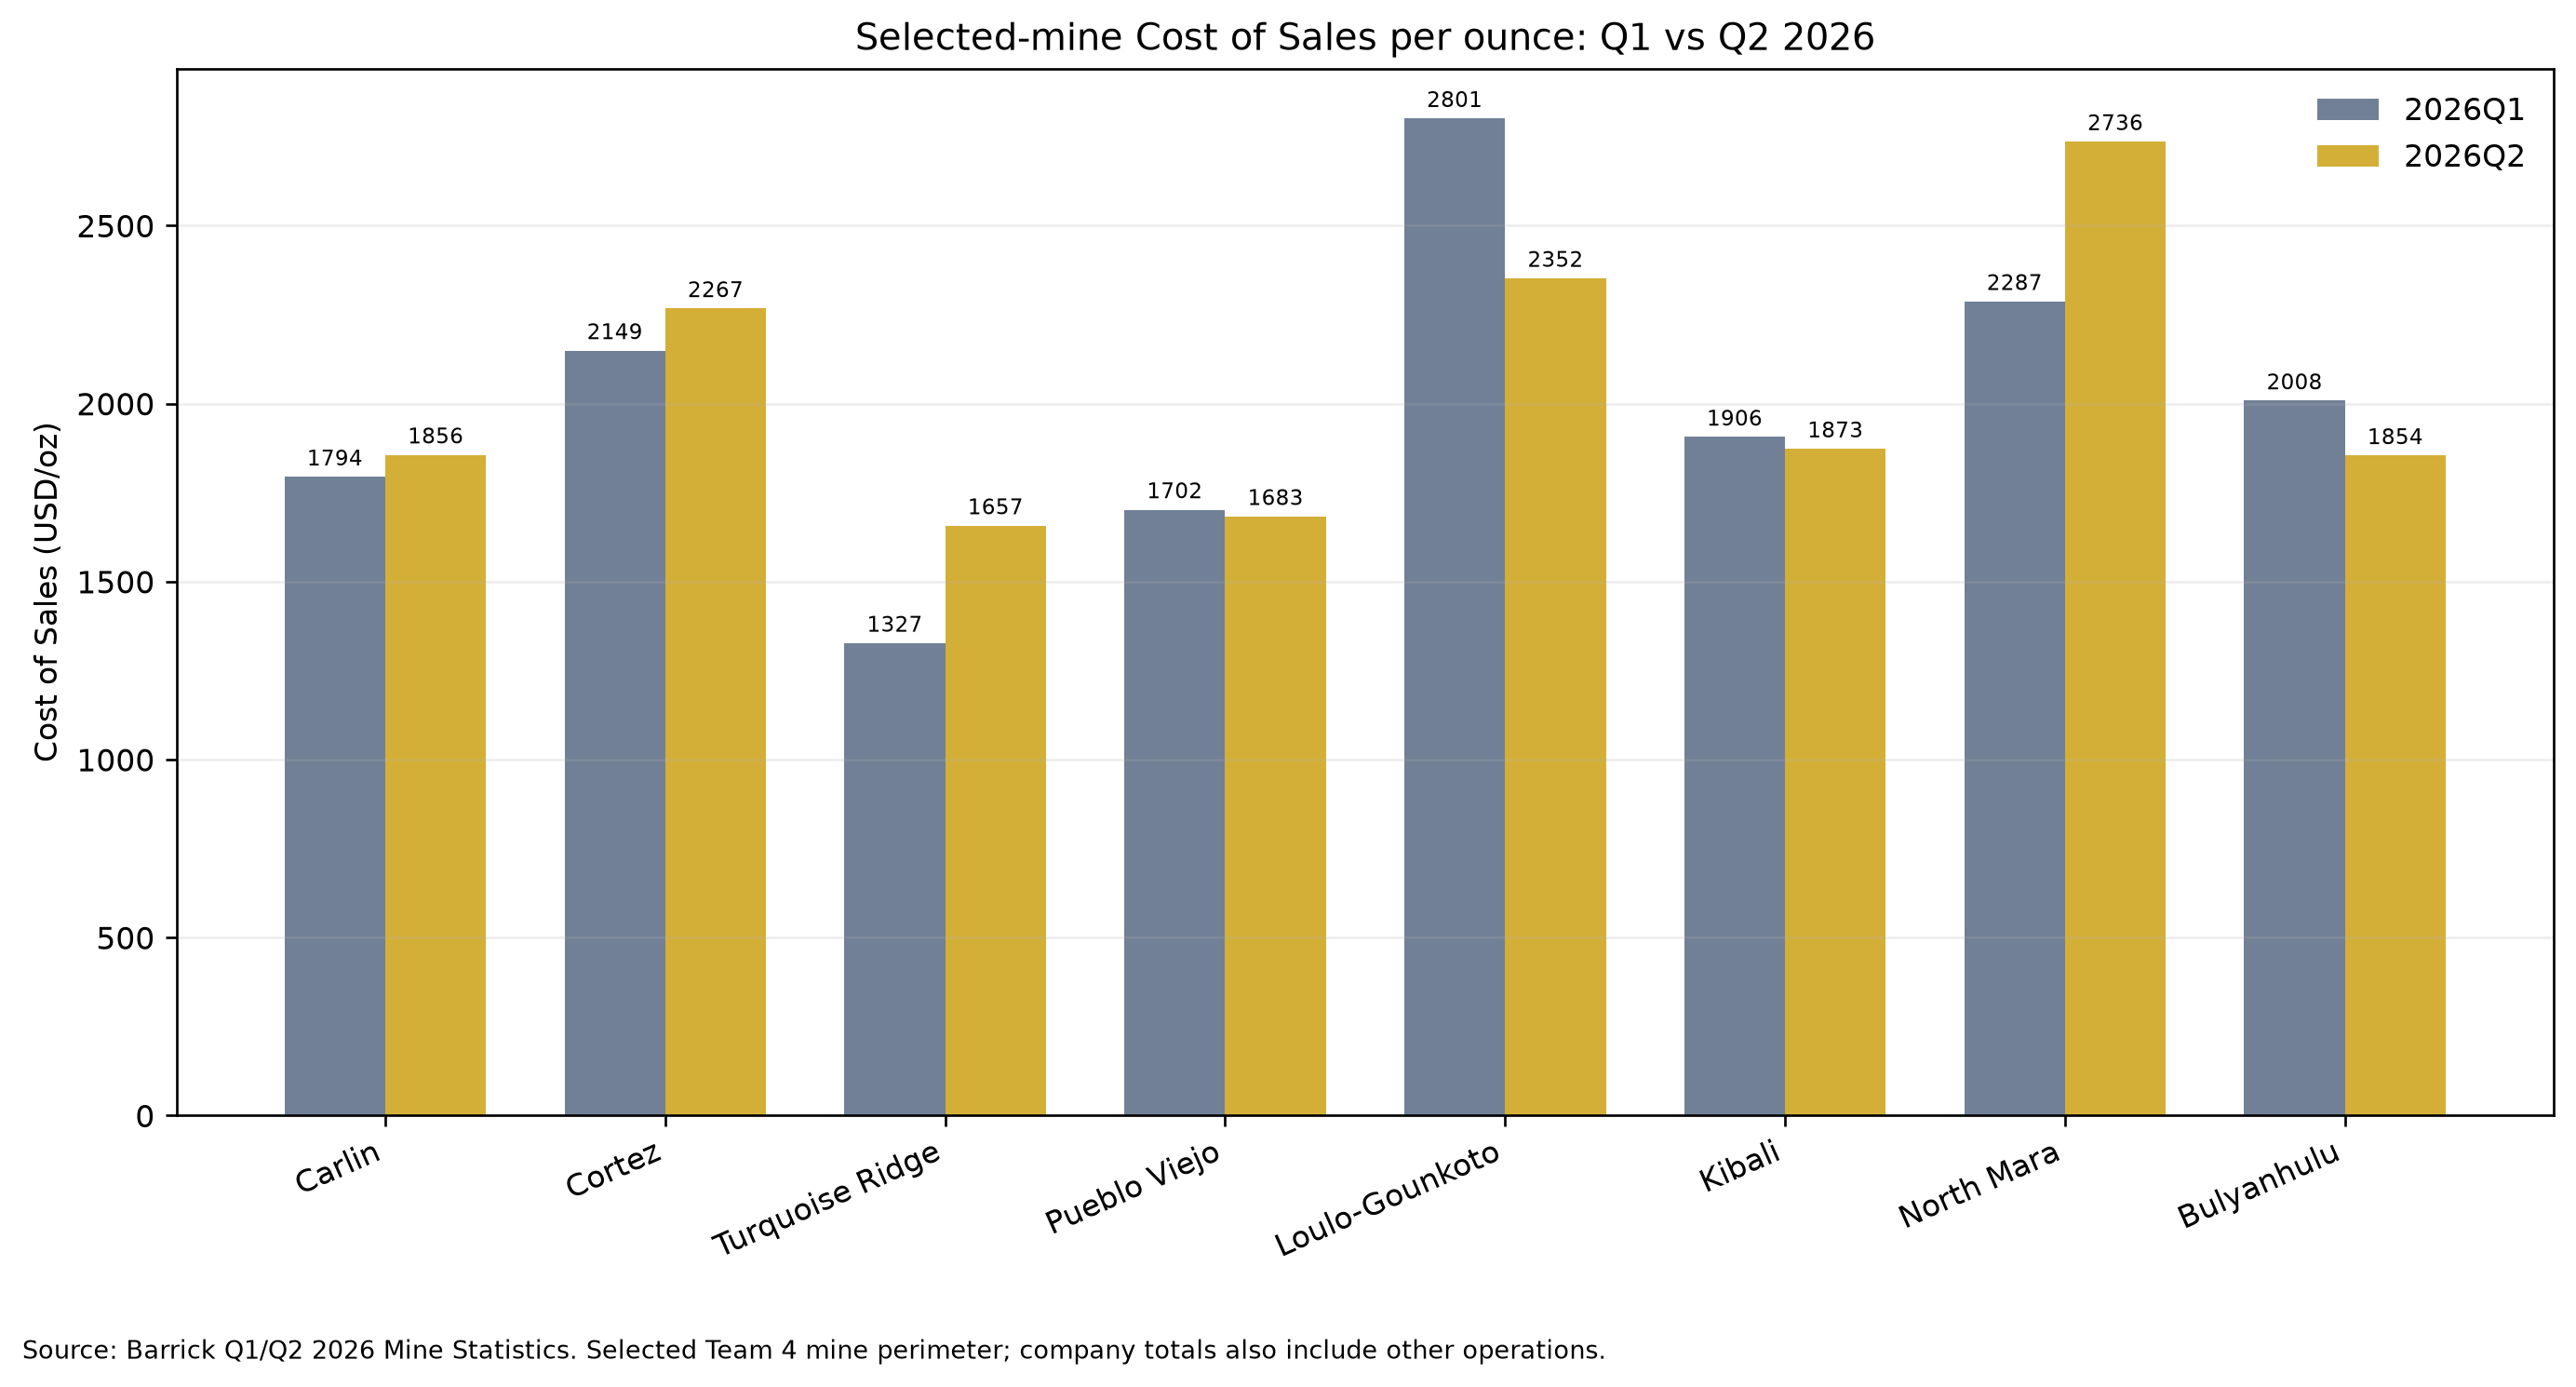
\includegraphics[width=0.95\columnwidth]{../img/publication/ce40d43c378d1fa2_team4_mine_cost_qoq.png}
  \captionof{figure}{Selected-mine Cost of Sales per ounce in Q1 and Q2 2026. Mine dispersion motivates preserving the Team 4 operating decomposition rather than replacing it with a single company-average cost.}
  \label{fig:team4_cost_qoq}
\par}
\end{minipage}\par

The scenario uses 20 fixed quarterly cost entries, including two 2026 actuals and 18 forecast entries. It does not propagate the source study's operating distributions.

\subsection{Production block}
Production is reconstructed from ore processed, grade and recovery using the specifications in Section~\ref{sec:paper-operating-models}. This preserves mine heterogeneity. The SARIMA orders are admitted from the source study, which does not report their selection by AIC/BIC.

\noindent\begin{minipage}{\columnwidth}
{\centering
  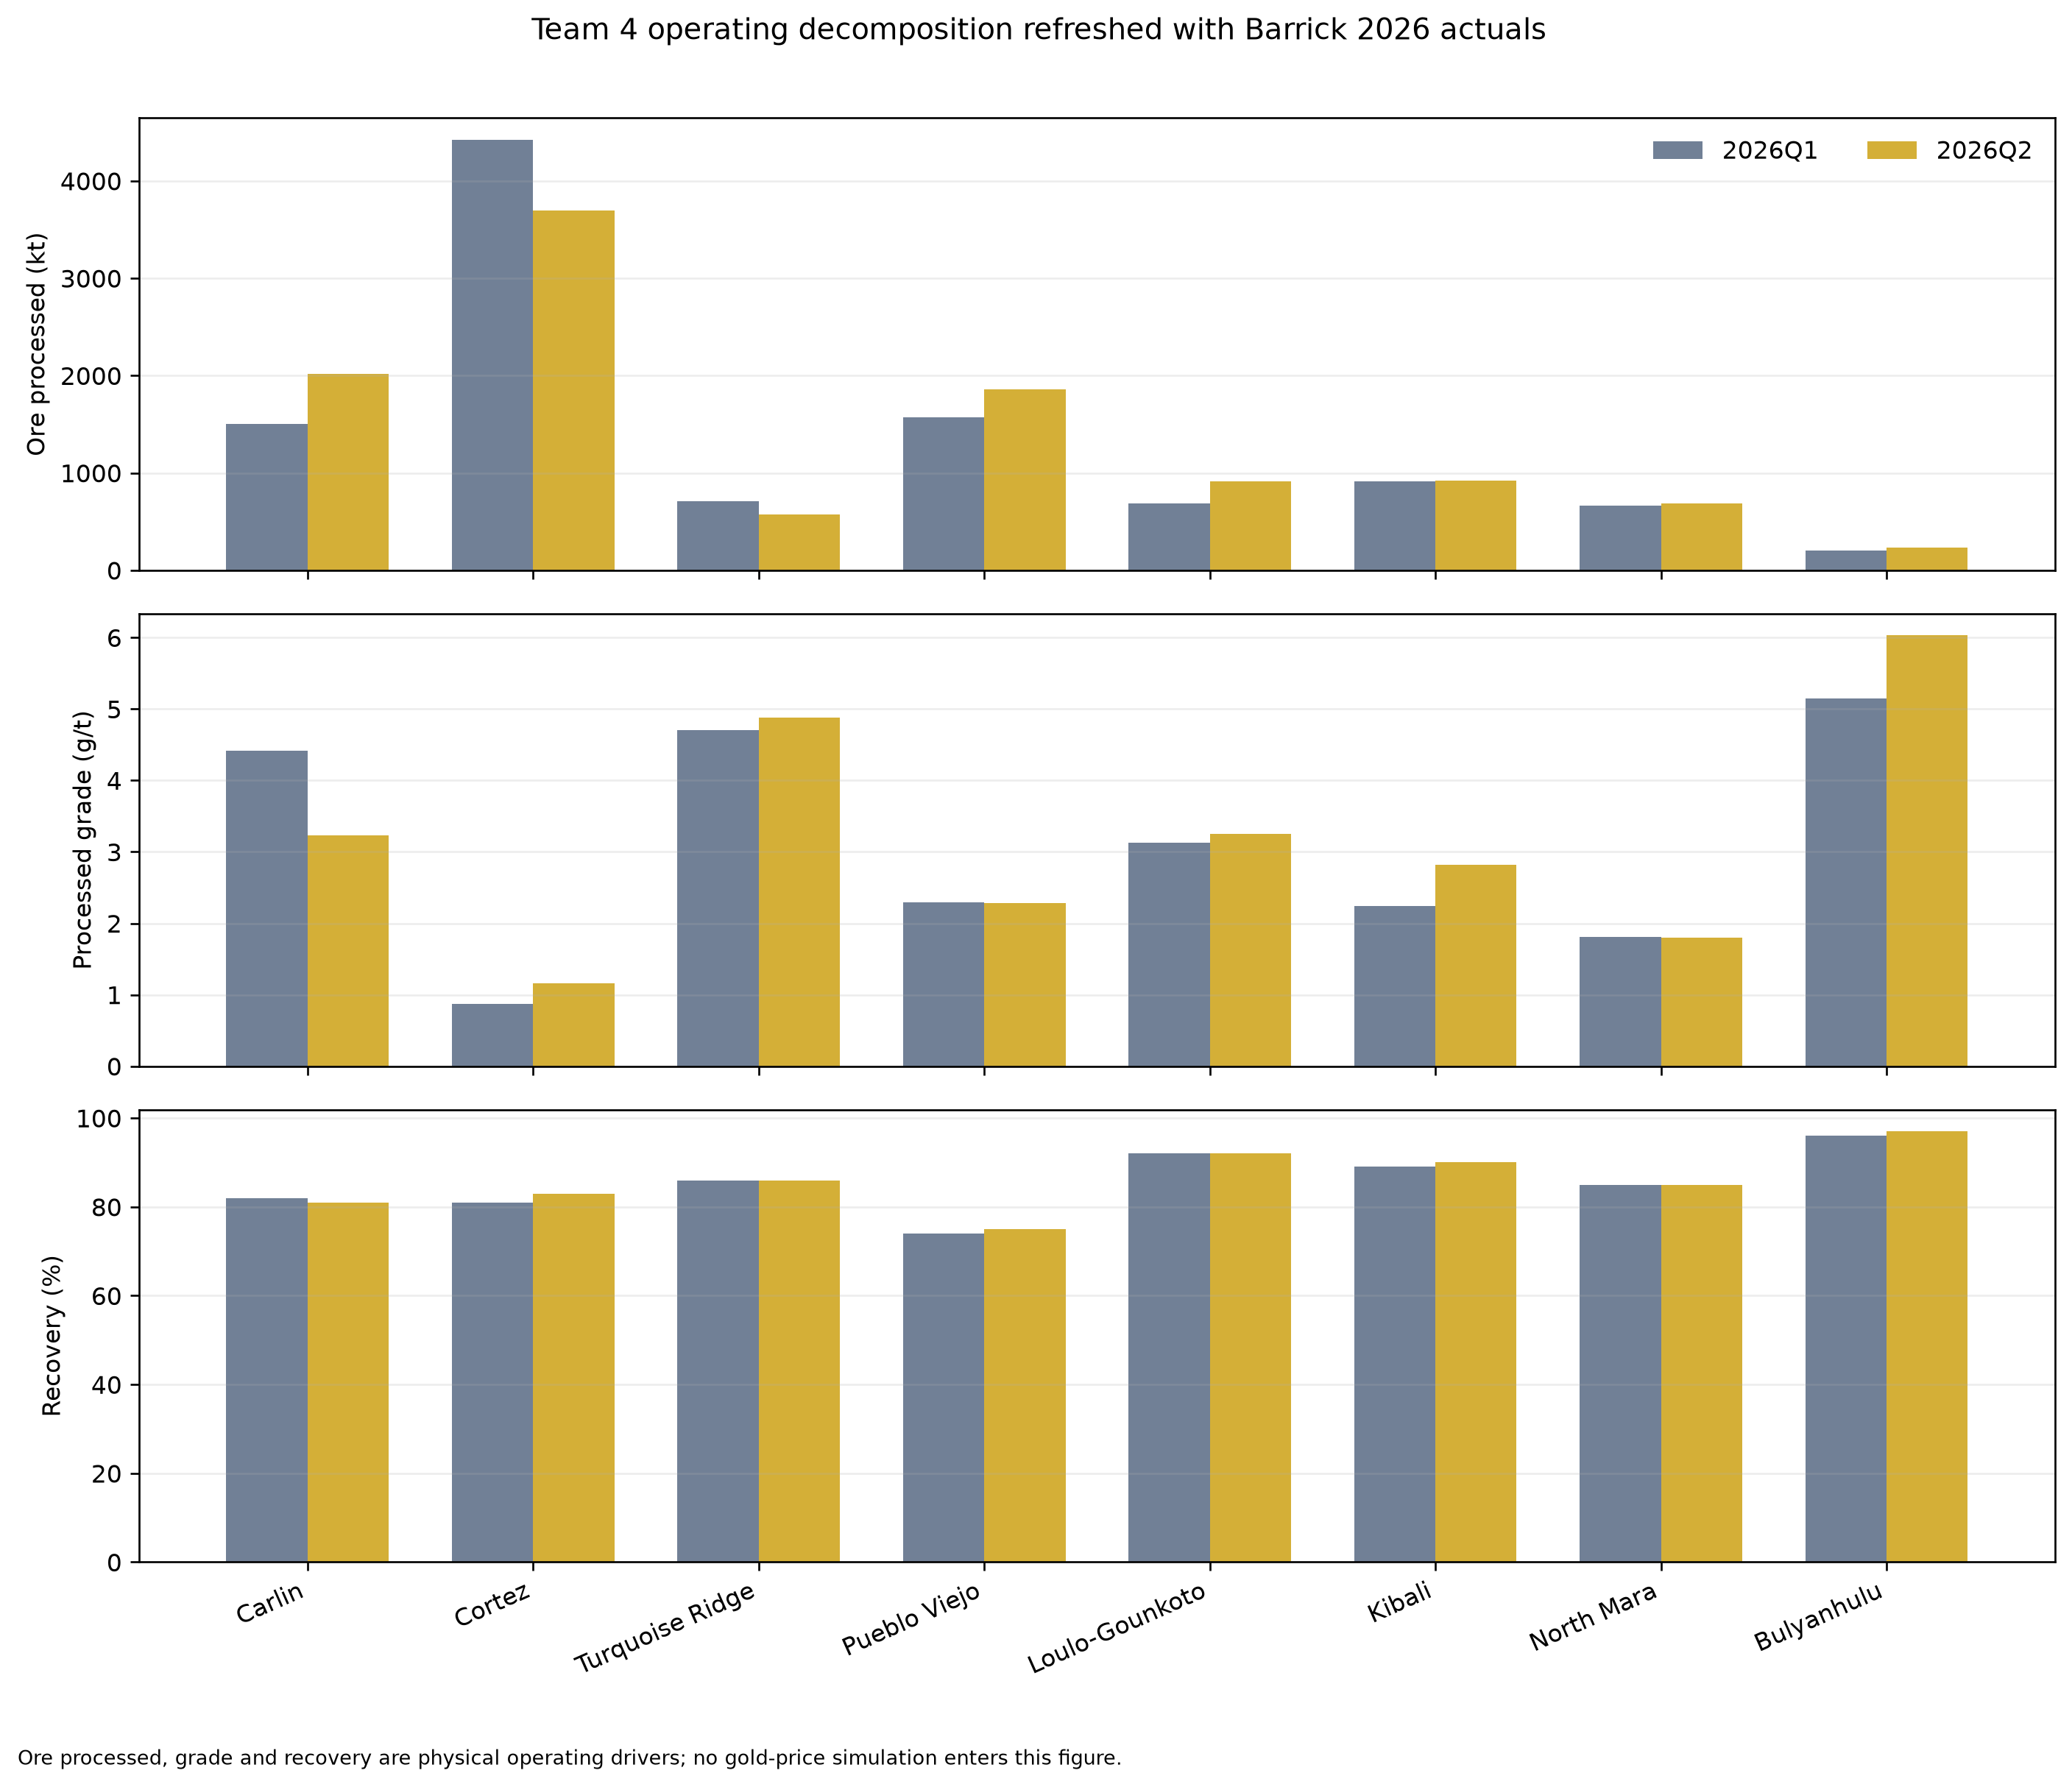
\includegraphics[width=0.95\columnwidth]{../img/publication/1ddc31b9d77b0ab4_team4_process_components_qoq.png}
  \captionof{figure}{Ore processed, grade and recovery updated with Barrick 2026 actuals. These are physical operating drivers; no commodity-price simulation enters the panel.}
  \label{fig:team4_process_qoq}
\par}
\end{minipage}\par

\noindent\begin{minipage}{\columnwidth}
{\centering
  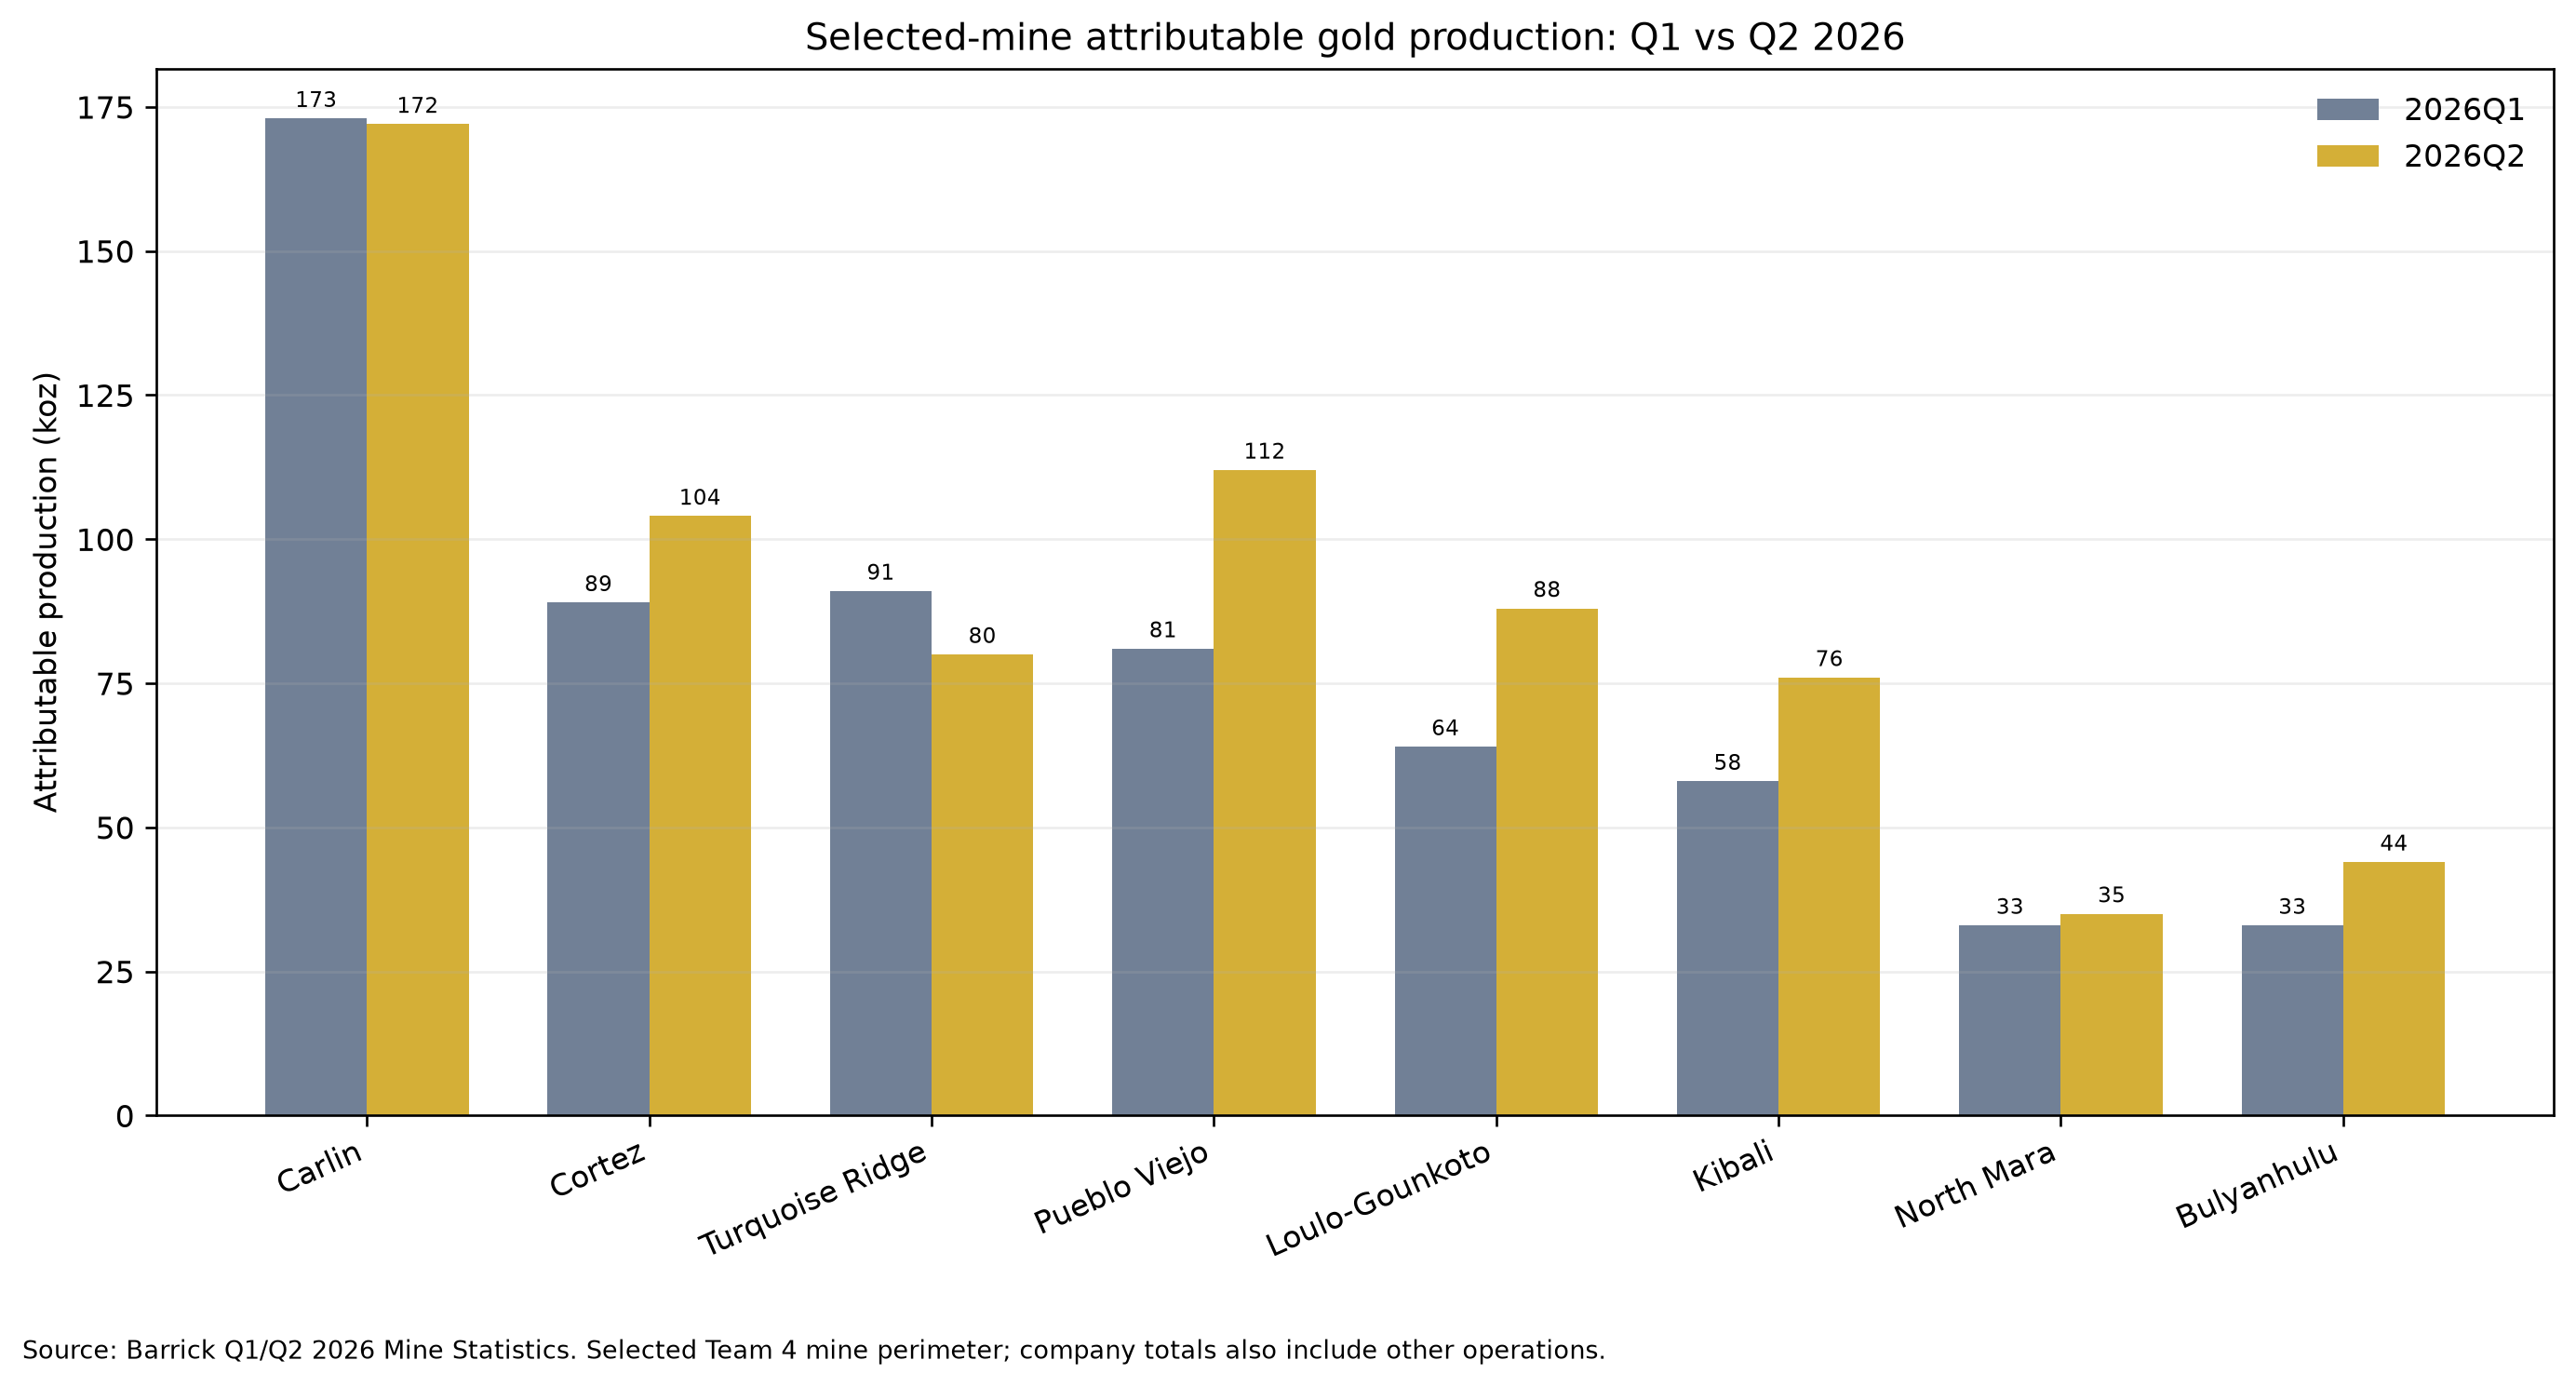
\includegraphics[width=0.95\columnwidth]{../img/publication/50b961f87c5f443e_team4_mine_production_qoq.png}
  \captionof{figure}{Selected-mine attributable gold production in Q1 and Q2 2026. The current actuals reveal heterogeneous changes that are hidden by a company-level total.}
  \label{fig:team4_production_qoq}
\par}
\end{minipage}\par

The original study also develops Goodman variance propagation and confidence bands for the production components. Those distributions remain useful evidence on operating-model uncertainty, but they are not propagated jointly in the four-engine corporate experiment: only the refreshed point vectors are passed downstream.

\subsection{Forecast handoff used by the valuation}
The final handoff keeps observed and modelled quantities distinct. Barrick's Q1--Q2 2026 actual production and CoS establish the current operating state; the Team 4 forecasts begin at Q3 2026 and extend through the common valuation horizon.

\noindent\begin{minipage}{\columnwidth}
{\centering
  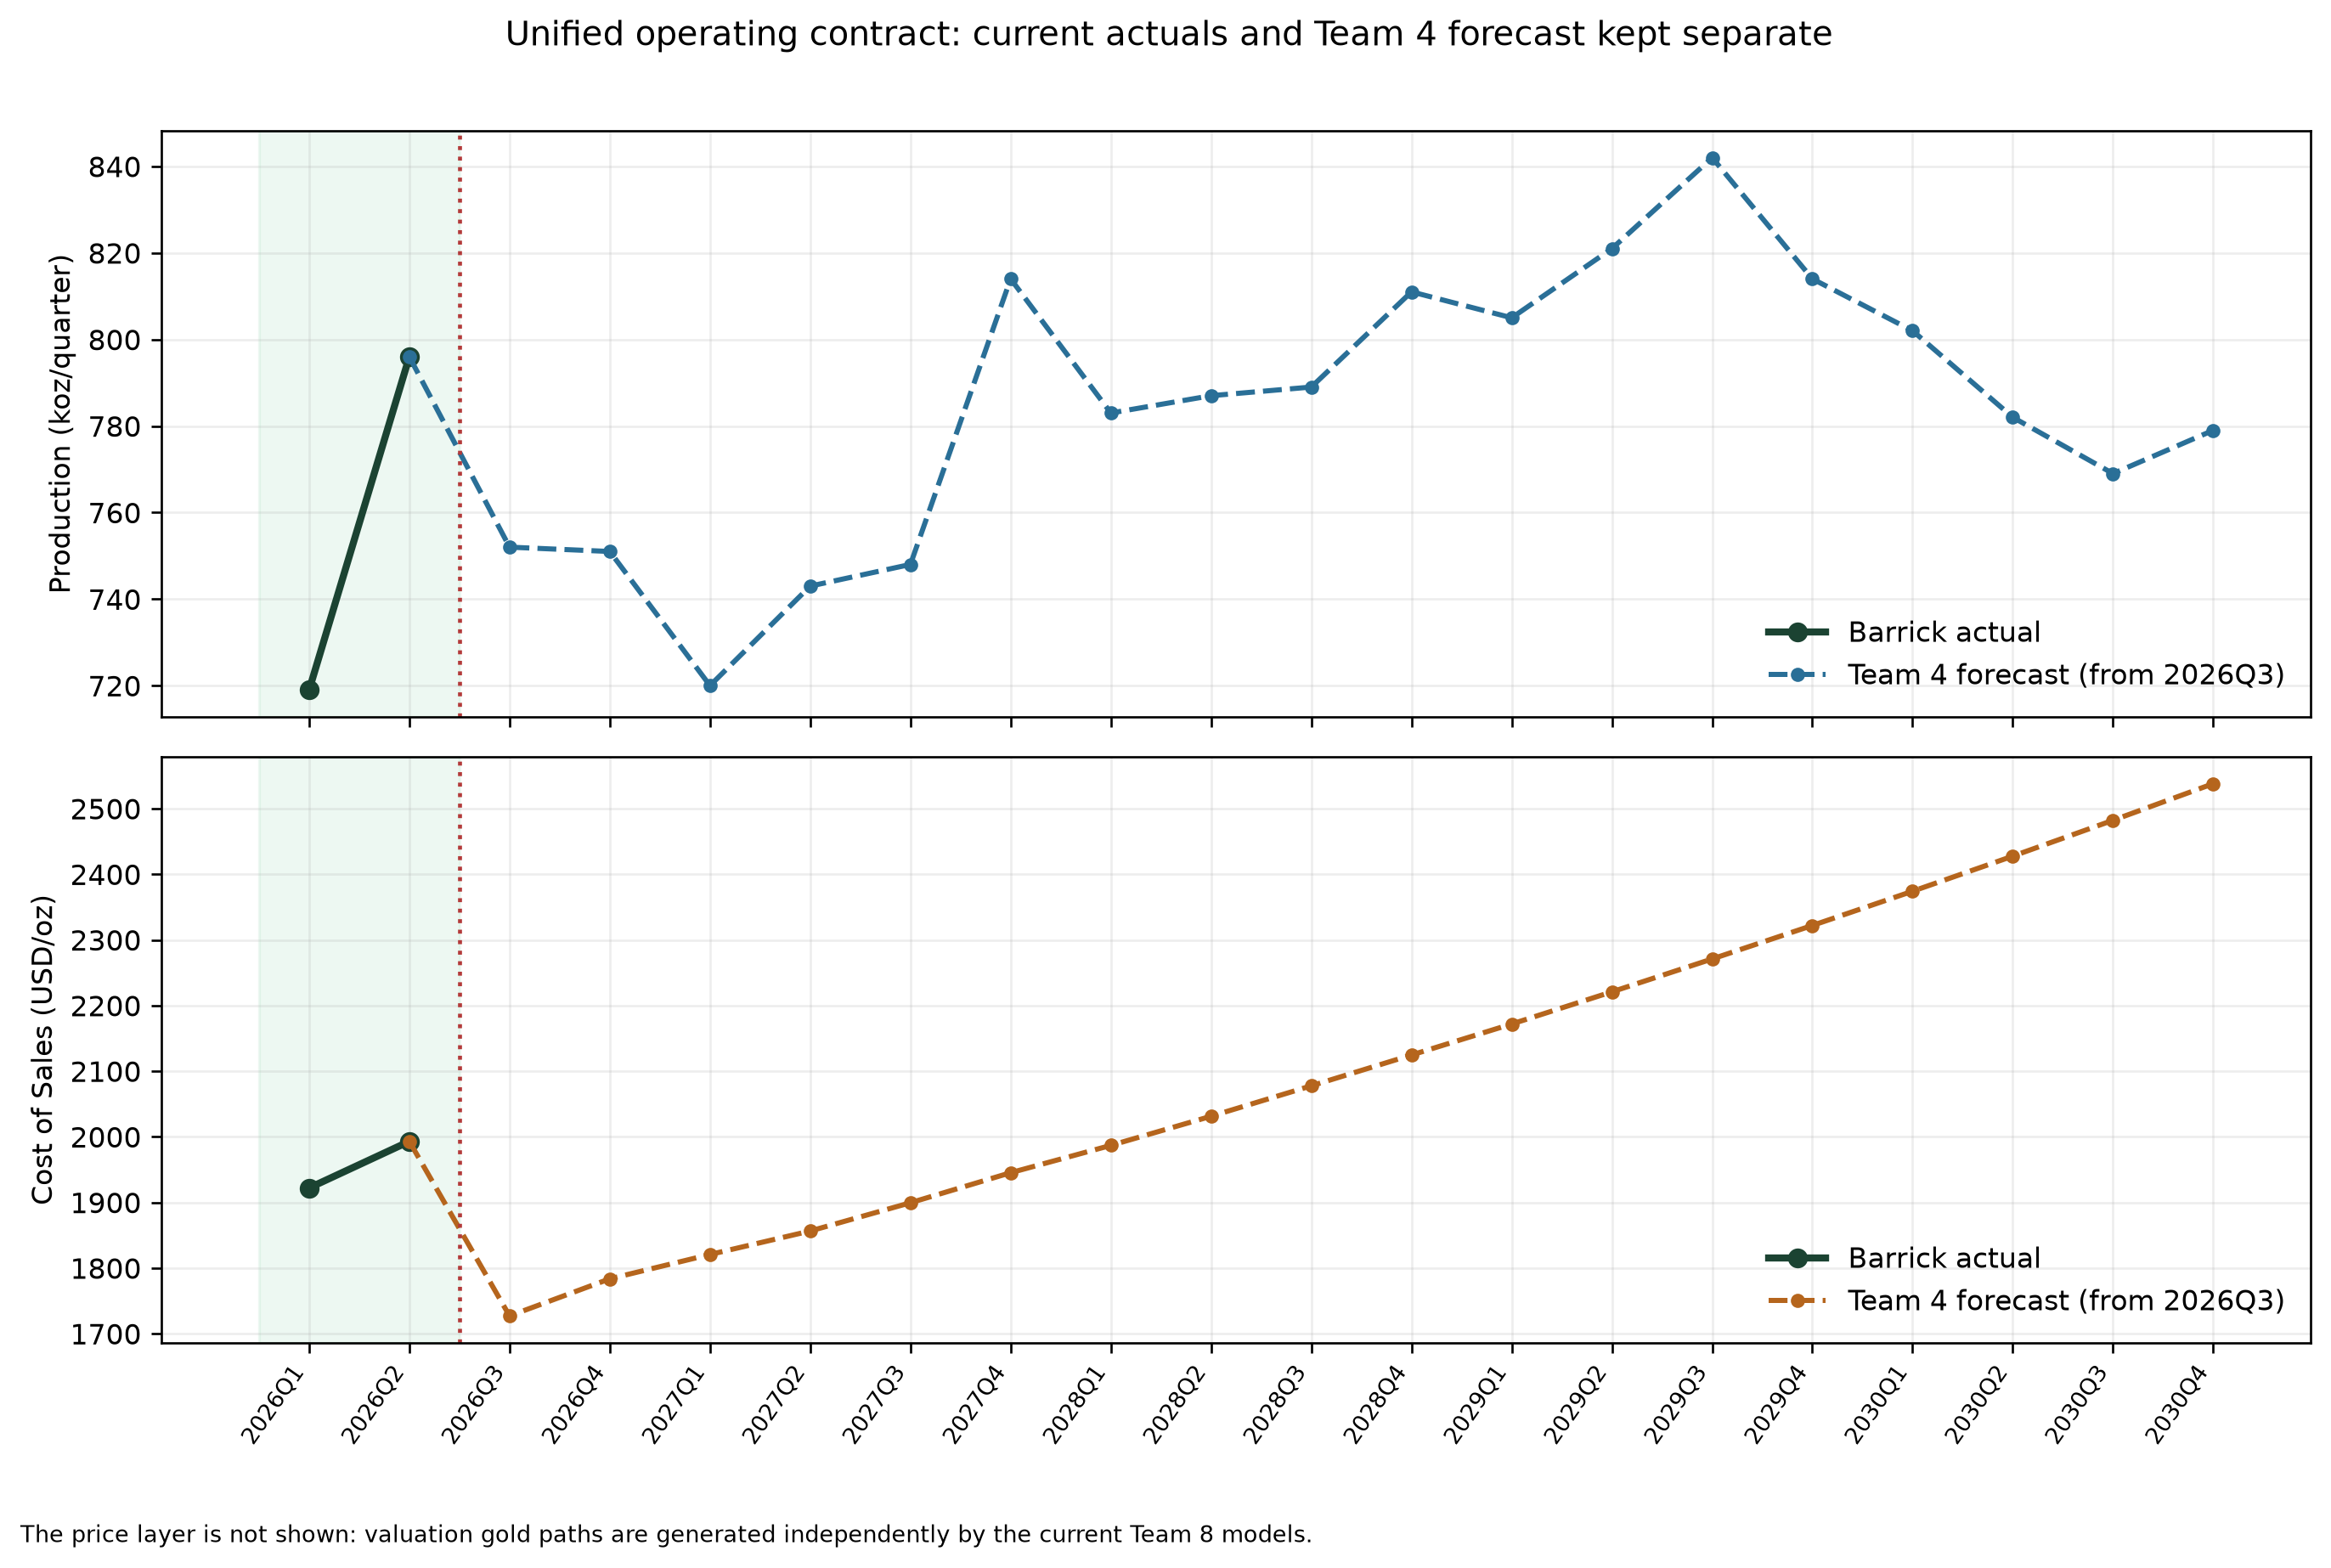
\includegraphics[width=0.95\columnwidth]{../img/publication/a5190673372d95dd_team4_operating_contract.png}
  \captionof{figure}{Inherited operating contract. Company-wide Q1--Q2 2026 actuals precede the eight-mine Team 4 forecast from Q3; the scope break is disclosed in Section 2.5. The straight cost path is the conditional mean of a persistent-trend specification, not a claim that operating uncertainty disappears.}
  \label{fig:team4_contract}
\par}
\end{minipage}\par

\begin{methodbox}[Prudential operating boundary]
Option-implied laws supply conditional scenario shapes to the proxy layer. Costs retain a persistent trend without additional technology-driven cost reductions. This is prudential relative to otherwise identical efficiency-improvement scenarios, but it does not establish a mathematical lower bound. Stochastic costs could yield favourable and adverse outcomes; the current fixed vectors preserve attribution across gold engines. Growth is already included in the common DCF schedule.
\end{methodbox}

\section{Calibration Sample Audit}

\noindent\begin{minipage}{\columnwidth}
{\centering
  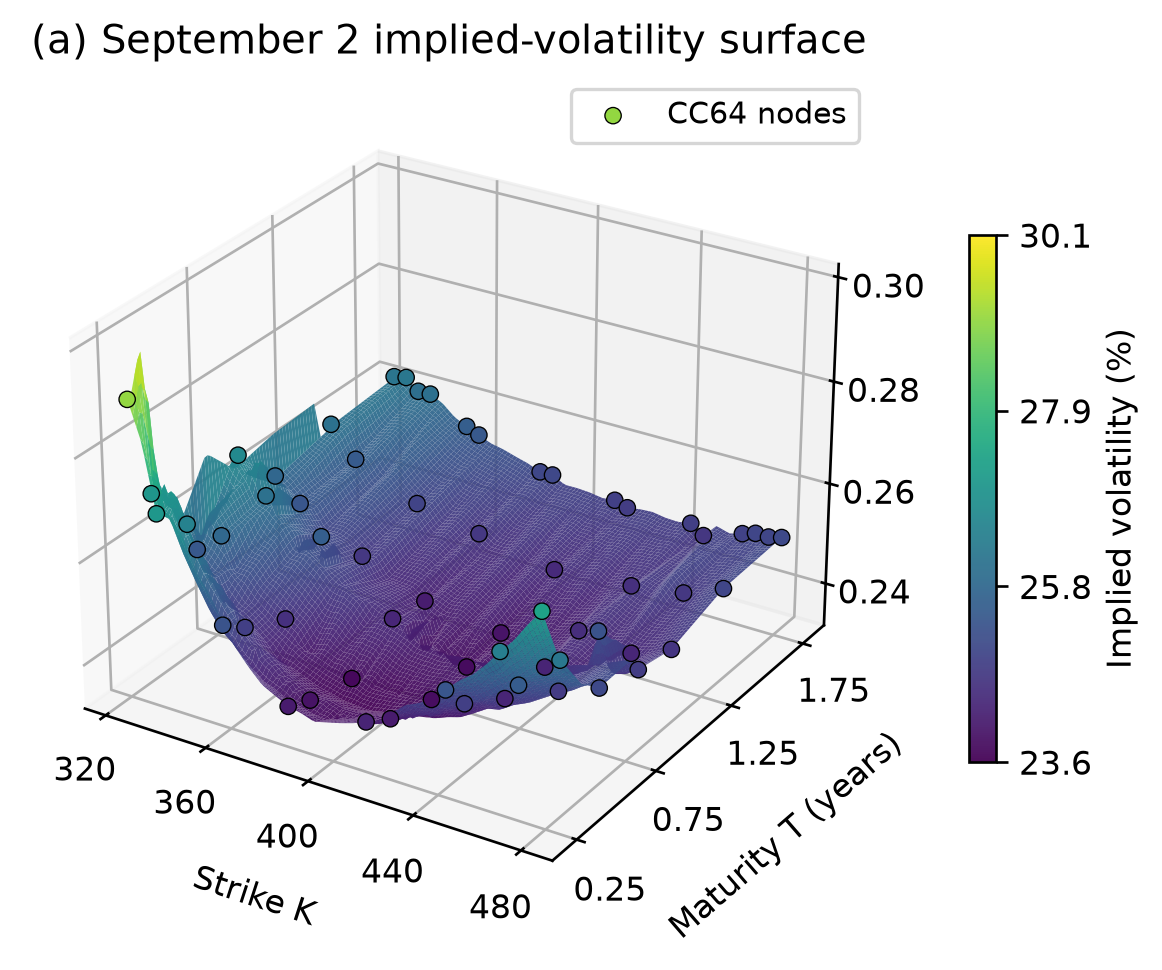
\includegraphics[width=\columnwidth]{../img/publication/6c5ba226b4a1f62f_sampling_surface_current.png}
  \captionof{figure}{(a) GLD implied-volatility surface, 2 September 2026, with CC64 nodes. Interpolation is used for display only.}
  \label{fig:chebyshev_audit}
\par}
\end{minipage}\par

\noindent\begin{minipage}{\columnwidth}
{\centering
  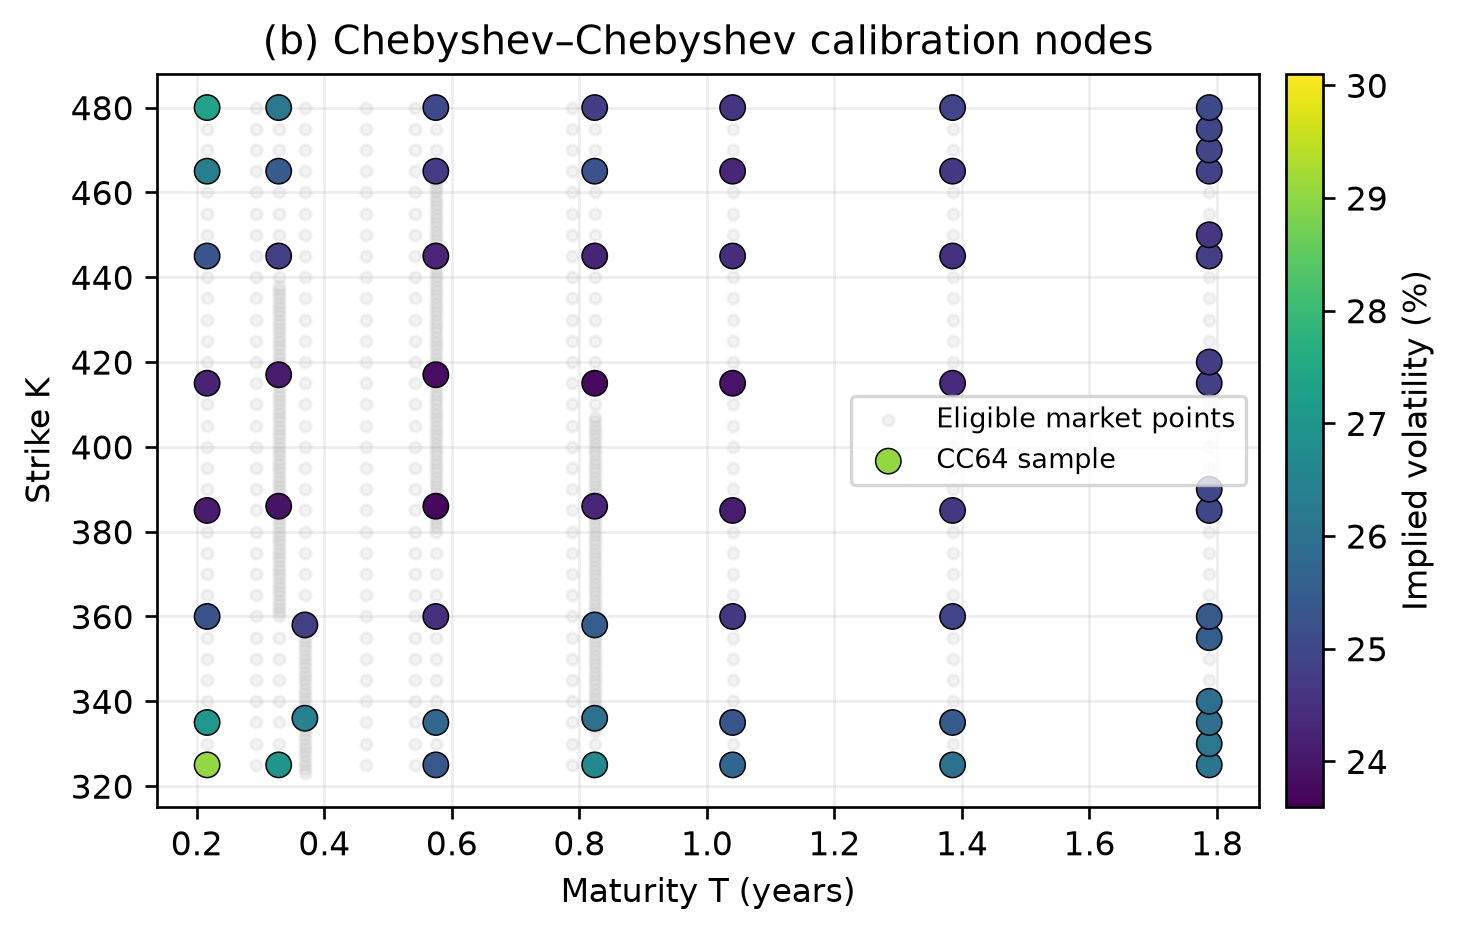
\includegraphics[width=0.95\columnwidth]{../img/publication/498fa63273eb3ac5_sampling_nodes.png}
  \captionof*{figure}{\textbf{Figure~\ref{fig:chebyshev_audit} (continued).} (b) The 64 actual contracts selected from 605 eligible calls across 12 expiries and 146 strikes.}
\par}
\end{minipage}\par

\subsection{Why structured sampling is retained}
The option surface is irregular in strike and maturity. Team 8 therefore passes a fixed $8\times8$ Chebyshev--Chebyshev subset to the optimizer rather than allowing densely listed regions to dominate the loss. Every target is mapped to the nearest still-unused actual option: the 64-point calibration set contains no synthetic contracts. The figure audits the same 2 September parameter snapshot used by the refreshed valuation.

\begin{methodbox}[Evidence status]
The residual maps, the parameters and the valuation paths come from one recalibration of the 2 September sample with $q=0.40\%$, dated 24 October 2026. The Treasury curve and the gold spot anchor are dated 2 September as well.
\end{methodbox}

\subsection{What the residual maps add}
The residual heatmaps show where each specification systematically over- or under-prices the observed implied-volatility surface. Black--Scholes leaves the strongest smile and term-structure pattern. Bates is refined from the nested Heston point and Bates--Hawkes from the nested Bates point, so each richer model fits at least as well as the model it contains (Table~\ref{tab:iv_rmse}). All maps use one colour scale; calibration fit does not establish economic superiority.

\noindent\begin{minipage}{\columnwidth}
{\centering
  \includegraphics[width=0.95\linewidth]{\FigBlackScholesResidualHeatmap}
  \par\vspace{1pt}{\footnotesize\textbf{(a)} Black--Scholes\par}
  \vspace{3pt}
  \includegraphics[width=0.95\linewidth]{\FigHestonResidualHeatmap}
  \par\vspace{1pt}{\footnotesize\textbf{(b)} Heston\par}
  \captionof{figure}{Implied-volatility residual maps for the common 2 September CC64 sample with $q=0.40\%$. Blue denotes model IV above market IV and red denotes model IV below market.}
  \label{fig:residual_maps}
\par}
\end{minipage}\par

\vspace{4pt}
\noindent\begin{minipage}{\columnwidth}
{\centering
  \includegraphics[width=0.95\linewidth]{\FigBatesResidualHeatmap}
  \par\vspace{1pt}{\footnotesize\textbf{(c)} Bates--Poisson\par}
  \vspace{3pt}
  \includegraphics[width=0.95\linewidth]{\FigBatesHawkesResidualHeatmap}
  \par\vspace{1pt}{\footnotesize\textbf{(d)} Full Bates--Hawkes\par}
  \captionof*{figure}{\textbf{Figure~\ref{fig:residual_maps} (continued).} Bates--Poisson and Full Bates--Hawkes residual maps; all colourbars share the same residual range.}
\par}
\end{minipage}\par

\begin{table}[H]
\centering
\caption{Current-surface IV calibration RMSE (bp). The 7 September column used $q=0$; the IV targets differ, so the columns are not a like-for-like fit comparison.}
\label{tab:iv_rmse}
\begin{tabular}{@{}lrr@{}}
\toprule
Model & $q=0.40\%$ & 7 Sep, $q=0$ \\
\midrule
Black--Scholes & \CalBSIVRMSE & \CalBSIVRMSELegacy \\
Heston & \CalHIVRMSE & \CalHIVRMSELegacy \\
Bates--Poisson & \CalBIVRMSE & \CalBIVRMSELegacy \\
Full Bates--Hawkes & \CalWIVRMSE & \CalWIVRMSELegacy \\
\bottomrule
\end{tabular}
\end{table}

\subsection{What the fit can and cannot identify}
With the fee as carry the fit deteriorates: the Heston price RMSE rises from USD~\CarryPriceRMSEZero{} to \CarryPriceRMSEFee{}, and the loss increases in every moneyness bucket. The calls therefore price a higher carry than Treasury rates less the fee. Call-only surfaces cannot separate that carry from skew, so a fitted carry would not be a forward; the futures-implied fee is used instead, and identifying the forward would need puts or box-spread rates.

\begin{methodbox}[Calibration fragility]
The Feller condition is imposed as a hard constraint and binds at the optimum for Bates and Bates--Hawkes; without it the Heston loss falls by \FellerRelaxedLossRatio\%. The Heston loss changes by less than 3\% for $\kappa$ between \KappaFlatLow{} and \KappaFlatHigh, so mean reversion is weakly identified. With $q=0.40\%$ the Bates jump intensity is \BatesLambda{} a year rather than zero, but jump and Hawkes parameters rest on 64 calls and are not individually identified. Bates--Hawkes branching is \HawkesBranching{} with a kernel half-life of \HawkesHalfLifeDays{} days.
\end{methodbox}

\section{DCF Driver and Terminal-Value Audit}

Growth, reinvestment, WACC and terminal closure are shared across gold engines. Table~\ref{tab:dcf_inputs} summarizes the corporate assumptions.

\subsection{Growth, ROIC and reinvestment}
Growth and ROIC converge linearly to their stable levels over the five rate years since valuation. Reinvestment follows $b_t=g_t/ROIC_t$, linking growth to the capital required to sustain it (Figure~\ref{fig:dcf_driver_schedule}).

\noindent\begin{minipage}{\columnwidth}
{\centering
  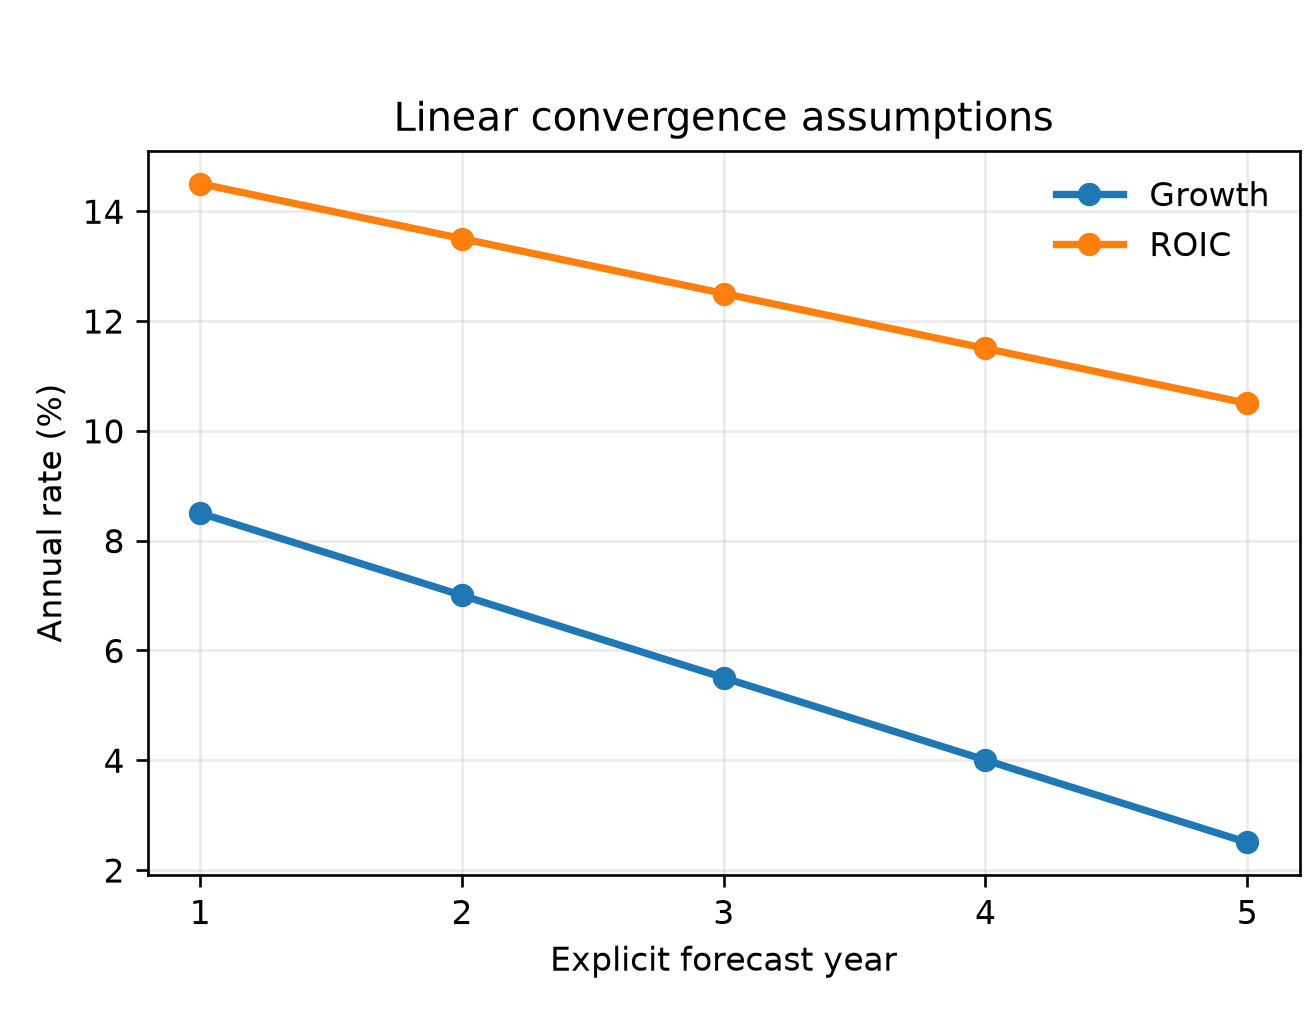
\includegraphics[width=0.90\linewidth]{../img/publication/ed4f022292eacd31_fig_dcf_growth_roic.png}
  \captionof{figure}{Common explicit-period DCF schedule: growth and ROIC converge linearly over the five-year horizon.}
  \label{fig:dcf_driver_schedule}
\par}
\end{minipage}\par

\noindent\begin{minipage}{\columnwidth}
{\centering
  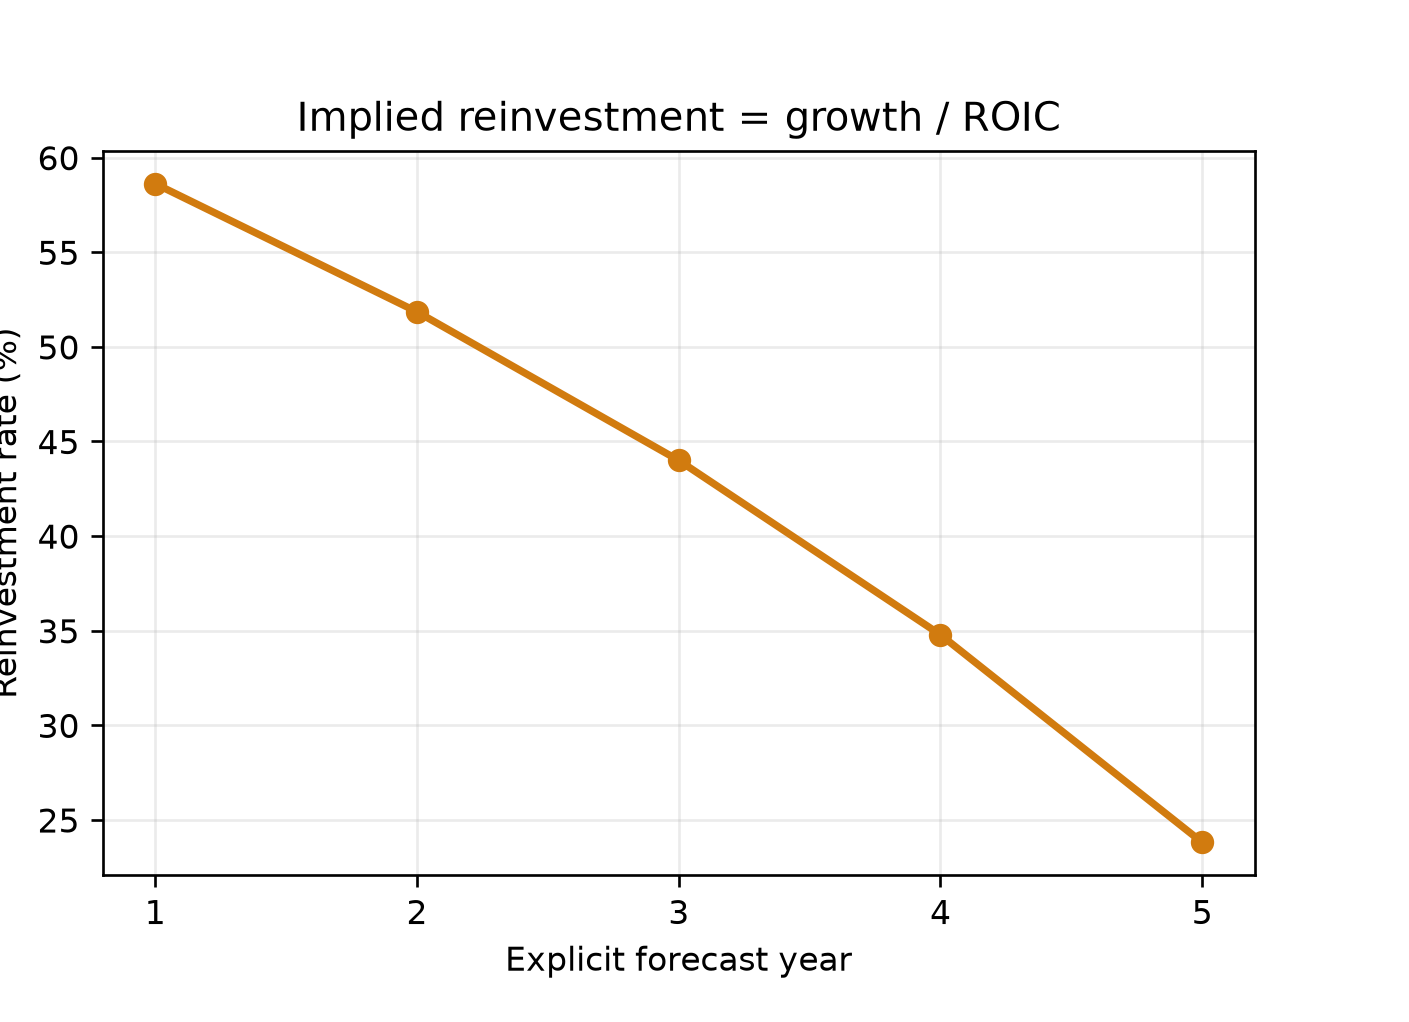
\includegraphics[width=0.90\linewidth]{../img/publication/ccbd1218e069545e_fig_dcf_reinvestment.png}
  \captionof*{figure}{\textbf{Figure~\ref{fig:dcf_driver_schedule} (continued).} The implied reinvestment rate, defined as growth divided by ROIC, falls from 58.62\% to 23.81\%.}
\par}
\end{minipage}\par

\subsection{Common stochastic WACC}
WACC follows the bounded mean-reverting process in Equation~\eqref{eq:wacc_process}, with inputs in Table~\ref{tab:dcf_inputs}; $w_0$ applies to the first year after valuation. Its annual innovation scale is $\sigma_w^*=\sigma_w\sqrt{(1-e^{-2\kappa_w})/(2\kappa_w)}=0.7308$ percentage points before clipping. All engines reuse the same 8,192 shock paths (Figure~\ref{fig:wacc_assumptions}).

\noindent\begin{minipage}{\columnwidth}
{\centering
  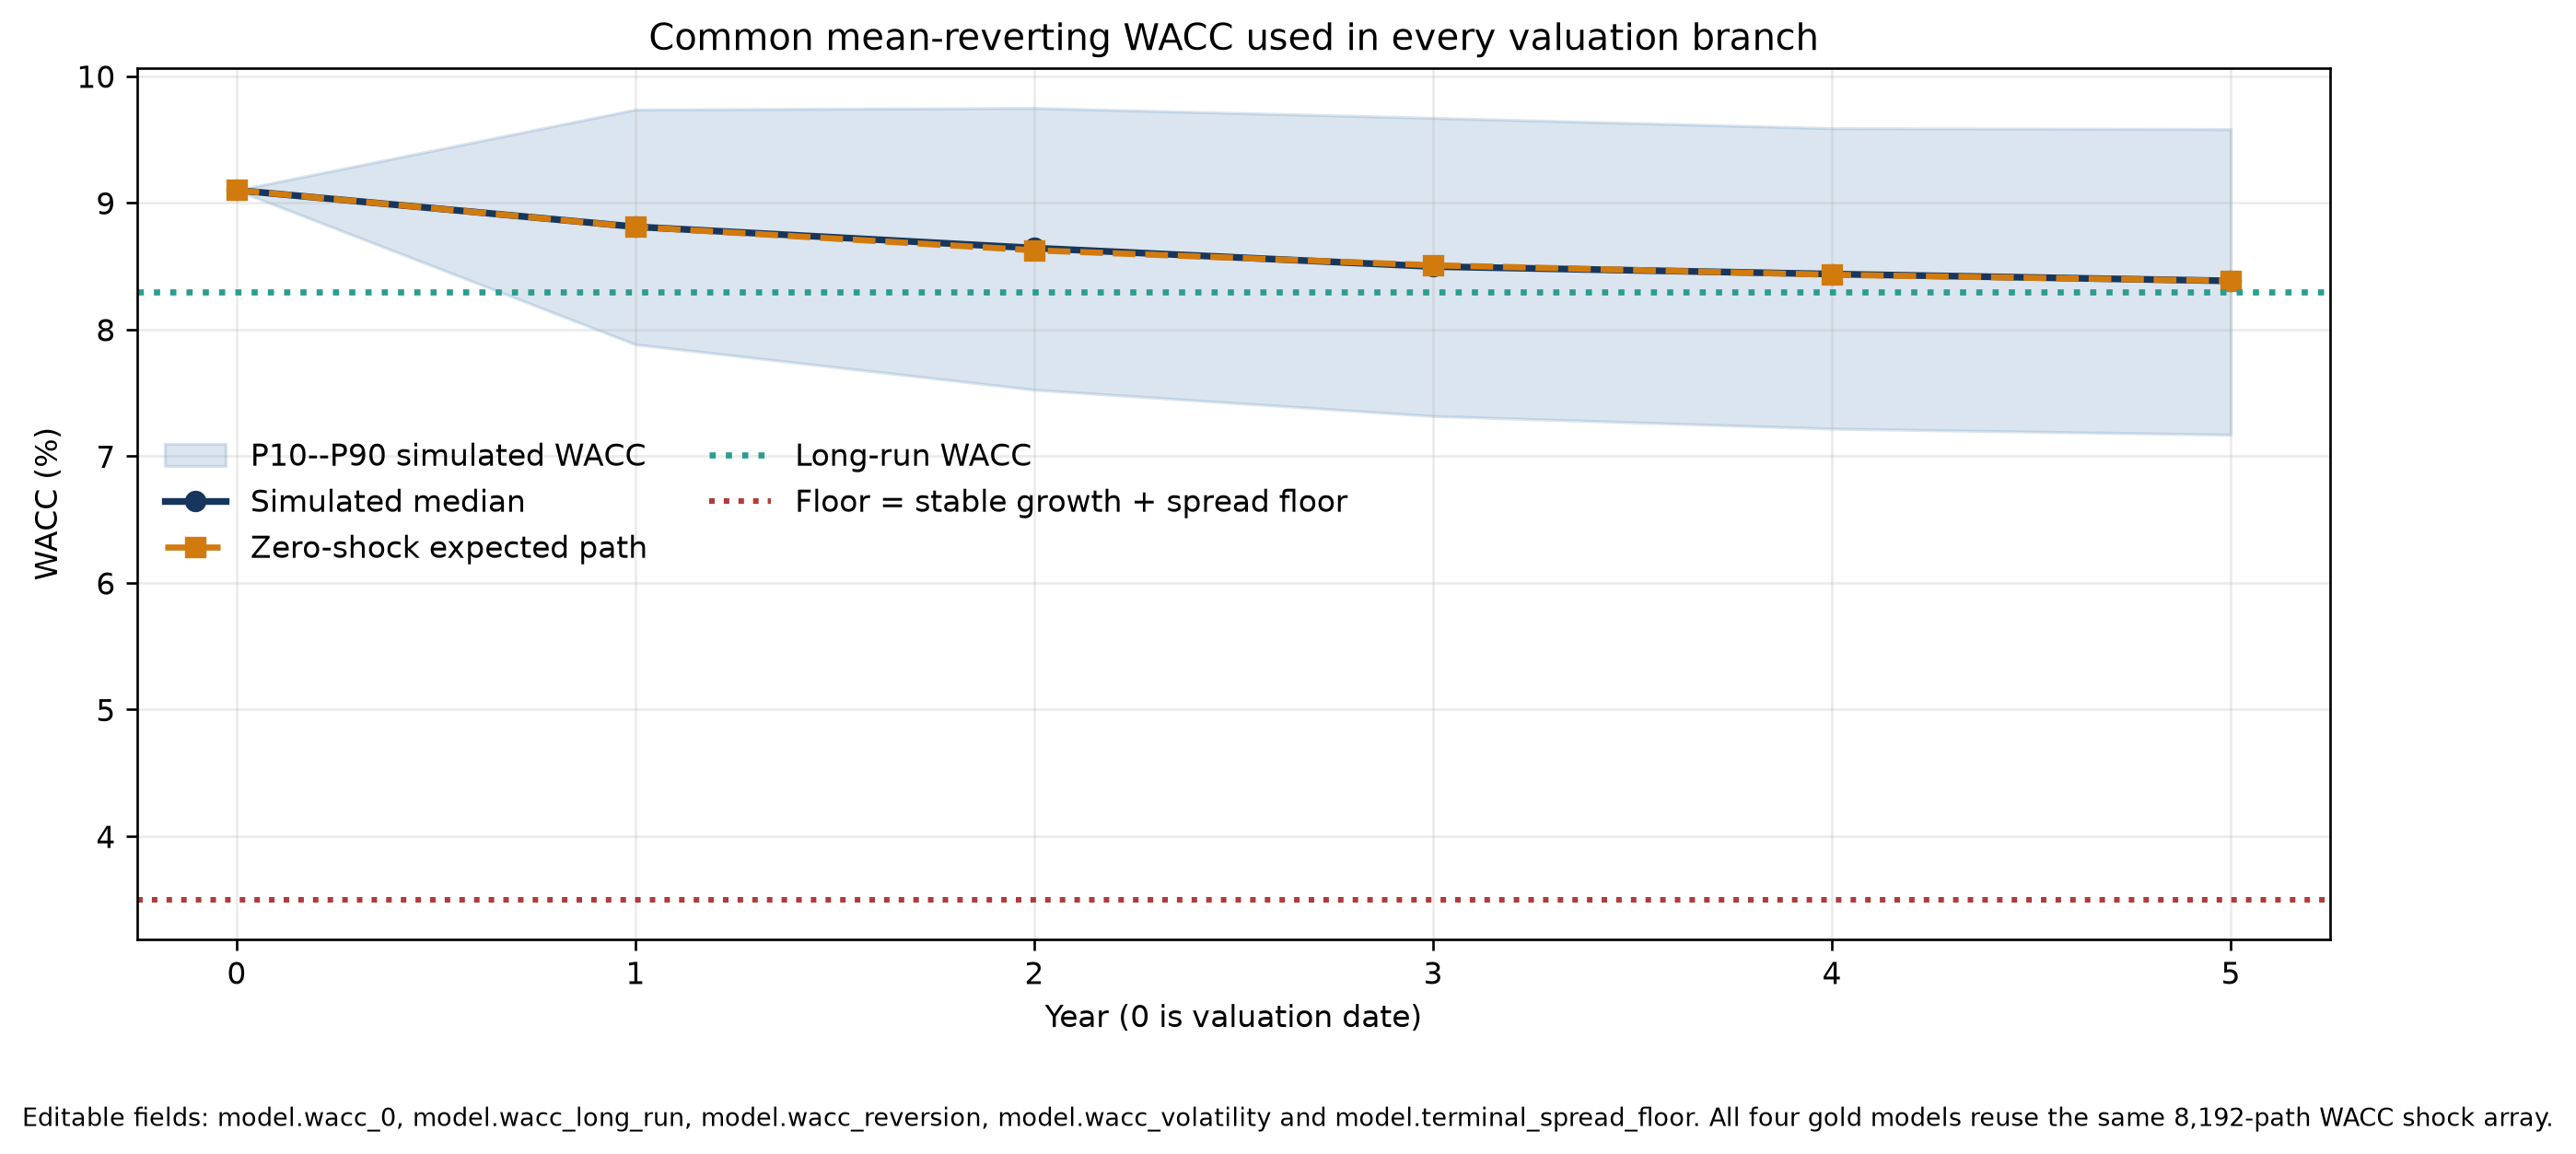
\includegraphics[width=0.95\columnwidth]{../img/publication/23df2023b1bd378f_fig_wacc_assumptions.png}
  \captionof{figure}{Common mean-reverting WACC. The band is the P10--P90 range from the shared 8,192-path shock array; the orange line is the zero-shock path and the dotted lines show the long-run level and admissibility floor.}
  \label{fig:wacc_assumptions}
\par}
\end{minipage}\par

\subsection{Terminal closure and sensitivity}
The terminal block uses $g_\infty=2.50\%$, $ROIC_\infty=10.50\%$ and terminal reinvestment of 23.81\%. At the median terminal WACC of \TerminalWACC\%, the terminal multiple is \TerminalMultiple$\times$ the final after-tax margin. The spread floor enforces $w_H>g_\infty$; \WACCClippedShare\% of simulated rates reach a clipping bound.

\noindent\begin{minipage}{\columnwidth}
{\centering
  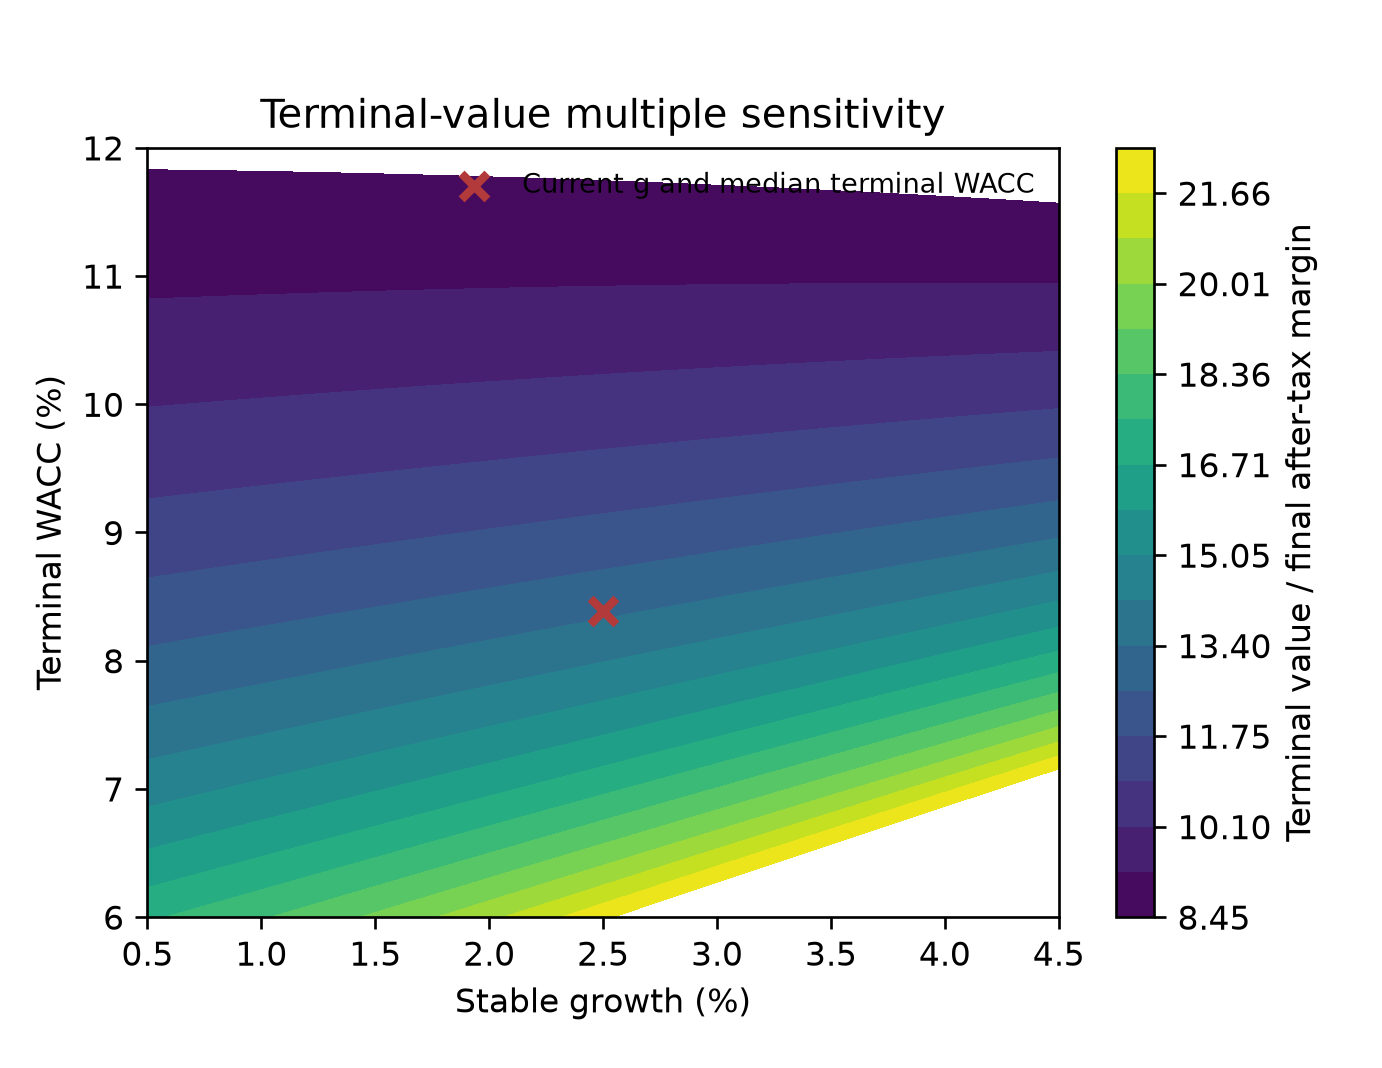
\includegraphics[width=0.90\linewidth]{../img/publication/2f2a7cea66301ac9_fig_terminal_multiple.png}
  \captionof{figure}{Terminal-value multiple sensitivity to stable growth and terminal WACC. The cross marks the configured stable-growth rate and current median terminal WACC.}
  \label{fig:terminal_value_mechanics}
\par}
\end{minipage}\par

\noindent\begin{minipage}{\columnwidth}
{\centering
  \includegraphics[width=0.90\linewidth]{\FigFigTerminalShare}
  \captionof*{figure}{\textbf{Figure~\ref{fig:terminal_value_mechanics} (continued).} Median proxy under the terminal conventions and with risk-free discounting of the explicit flows. Explicit flows to 2030 are worth about USD~11 billion against about USD~57--59 billion with a perpetuity. Zero terminal is a truncation scenario, not an estimated reserve life.}
\par}
\end{minipage}\par

\begin{table}[H]
\centering
\caption{Editable common DCF inputs.}
\label{tab:dcf_inputs}
\begin{tabularx}{\columnwidth}{@{}Xr@{}}
\toprule
Parameter & Value \\
\midrule
Tax rate & 25.00\% \\
$g_1\rightarrow g_\infty$ & 8.50--2.50\% \\
$ROIC_1\rightarrow ROIC_\infty$ & 14.50--10.50\% \\
$WACC_0\rightarrow\bar w$ & 9.10--8.30\% \\
WACC reversion & 0.45 \\
WACC volatility & 0.90\% \\
WACC floor/cap & 3.50/25.00\% \\
Terminal reinvestment & 23.81\% \\
\bottomrule
\end{tabularx}
\end{table}

\begin{methodbox}[Interpretation]
These are methodological assumptions, not filing-calibrated Barrick estimates. Terminal closure dominates the reported operating proxy: it accounts for about \TerminalShare\% of the mean. The former positive floor on the final margin is no longer used; it leaves medians unchanged.
\end{methodbox}

The quarterly bridge multiplies the average simulated gold price less unit Cost of Sales, both in USD per ounce, by production in thousand ounces, then divides by 1,000 to obtain component margin in USD millions. Each quarter is taxed, charged its reinvestment and discounted at its own date. This proxy is not reported EBIT or FCFF: production must be reconciled with sales and inventory, and depreciation, capital expenditure and working capital must enter without double counting. Fixed operating vectors exclude mine-level shocks and price-cost dependence.

\section{Operating-Proxy Sensitivities}
\label{sec:results}

\begin{table}[H]
\centering
\caption{Bates--Hawkes operating proxy, USD billion unless stated.}
\label{tab:primary_signal}
\begin{tabularx}{\columnwidth}{@{}Xr@{}}
\toprule
Metric & Value \\
\midrule
P10 & \ValWPTen \\
Median (P50) & \ValWMedian \\
P90 & \ValWPNinety \\
Mean & \ValWMean \\
Negative proxy paths & \ValWNegative\% \\
Explicit flows to 2030, median & \ValWExplicit \\
Same, risk-free discounting & \ValWExplicitRiskFree \\
\bottomrule
\end{tabularx}
\end{table}

\begin{findingbox}[Interpretation]
These are unconstrained aggregate operating proxies, not enterprise or equity values. Negative outcomes are not negative limited-liability share prices, and no market comparison is made.
\end{findingbox}

\noindent\begin{minipage}{\columnwidth}
{\centering
  \includegraphics[width=0.95\columnwidth]{\FigFigValPrimary}
  \captionof{figure}{Signed-terminal operating proxy under Bates--Hawkes on the dated clock, 8,192 paths. Display limits are the 0.5th--99.5th percentiles; the full tails remain in the data. This is not a confidence interval or a physical probability law.}
  \label{fig:value_distribution}
\par}
\end{minipage}\par

\subsection{Model choice matters less than numerical noise}
Medians range from USD~\ValMedianLow{} to \ValMedianHigh~billion across the four engines and P90 from \ValPNinetyLow{} to \ValPNinetyHigh. Doubling the paths to 16,384 or changing the seed moves single-model medians across USD~\NumericalMedianLow--\NumericalMedianHigh~billion; for Bates--Hawkes alone the range is \NumericalHawkesLow--\NumericalHawkesHigh. The numerical range of one model is as wide as the spread between models, so the four medians do not rank the models. Explicit flows to 2030 are worth USD~\ValExplicitLow--\ValExplicitHigh~billion and the terminal value carries about \TerminalShare\% of the mean.

\begin{table}[H]
\centering
\caption{Proxy medians, USD billion. Explicit: flows to 31 December 2030 without terminal value.}
\label{tab:model_comparison}
\begin{tabular}{@{}lrr@{}}
\toprule
Gold engine & Median & Explicit \\
\midrule
Black--Scholes & \ValBSMedian & \ValBSExplicit \\
Heston & \ValHMedian & \ValHExplicit \\
Bates--Poisson & \ValBMedian & \ValBExplicit \\
Full Bates--Hawkes & \ValWMedian & \ValWExplicit \\
\bottomrule
\end{tabular}
\end{table}

\subsection{What the corrections changed}
Table~\ref{tab:attribution} applies the corrections of this revision one at a time to the 7 September medians. The dated clock removes Barrick's first-half 2026 margin, which the earlier version discounted as a future flow, and ends the explicit horizon at 2030; between the two editions the explicit flows fall from about USD~13 to 11~billion. Each step moves the medians by less than the numerical range above.

\begin{table}[H]
\centering
\caption{Median proxy, USD billion, as each correction is added.}
\label{tab:attribution}
\begin{tabular}{@{}lrrrr@{}}
\toprule
Step & BS & Heston & Bates & B--H \\
\midrule
7 Sep Paper & \AttLegacyBS & \AttLegacyH & \AttLegacyB & \AttLegacyW \\
+ dated clock & \AttClockBS & \AttClockH & \AttClockB & \AttClockW \\
+ spot anchor & \AttAnchorBS & \AttAnchorH & \AttAnchorB & \AttAnchorW \\
+ GLD carry & \AttCarryBS & \AttCarryH & \AttCarryB & \AttCarryW \\
\bottomrule
\end{tabular}
\end{table}

\subsection{Structural illustration, not model selection}
Bates--Hawkes illustrates the richest law, not a preferred corporate valuation. Its branching ratio is \HawkesBranching{} and its kernel half-life $\log(2)/\beta$ is \HawkesHalfLifeDays{} days. These are risk-neutral fitted parameters, not measured geopolitical persistence.

\noindent\begin{minipage}{\columnwidth}
{\centering
  \includegraphics[width=0.95\columnwidth]{\FigFigValMulti}
  \captionof{figure}{Operating-proxy distributions under four gold-price laws. Operations, WACC and signed terminal closure are common. No share count, equity bridge or market reference is used.}
  \label{fig:multimodel_value_overlay}
\par}
\end{minipage}\par

\section{Copper Extension: History and Paired Operating Values}
\label{sec:copper-extension}

\subsection{Perimeter and units}
The original gold-only study omitted copper. The extension admits three producing mines: Lumwana (100\%), Zald\'ivar (50\%) and Jabal Sayid (50\%). Their Q2 2026 attributable sales are 40, 9 and 5 kt, and Cost of Sales is 3.14, 4.89 and 2.63 USD/lb, respectively \citep{barrickmine2026}. The sales quantities already incorporate ownership; multiplying by those shares again would understate the two joint ventures. Lumwana is consolidated, while the other two interests are equity-accounted \citep{barrickar2025}. Production and sales are distinct quantities; the copper margin uses sales.

With $s_i$ in kt and $P_t,c_i$ in USD/lb, quarterly attributable component margin in USD millions is
\begin{equation}
CM^{Cu}_t=\frac{2204.6226218488}{1000}\sum_i s_i(P_t-c_i).
\label{eq:copper-margin}
\end{equation}
Q2 sales and costs are held fixed for 20 quarters. This is a controlled operating scenario, not a mine-production forecast. CoS includes depreciation; reported capital expenditure is not separately deducted in this proxy. Expansion at Lumwana, Reko Diq, other gold assets, reserves and closure obligations remain outside the model.

\subsection{Historical surface and exercise treatment}
The IB API collection selected ten historical dates between 9 July and 2 September 2026 before scoring. Each date used 112 uniformly spaced out-of-the-money contract locations, rather than thousands of quotes. There are 912 returned quote rows across the pilot; missing responses are not fabricated. The common admission rule requires at least 64 eligible observations and three expiries, option and matched-future quote ages no greater than 120 seconds, and a relative option spread no greater than 20\%. Seven dates survive, creating six origin--target pairs with gaps of 11, 23, 9, 10, 1 and 1 calendar days. July 10, July 31 and August 3 fail the quality gate. Historical data therefore exist, but this is a sparse pilot rather than a daily panel; the other gold reference dates were not collected in this experiment.

Copper is quoted in USD/lb through COMEX HG futures and their American options. A 600-step constant-volatility CRR inversion removes the early-exercise convention before fitting European forward-price engines; a 300-step comparison checks discretization. This transformation does not solve early exercise under the full stochastic-volatility/jump models. Each option is matched to its own underlying future; Black--76 is the constant-volatility benchmark. Origin calibration uses the dated Treasury curve, with no target-date quote entering parameter selection. The 2 September current fit uses all 86 eligible observations.

\subsection{Temporal tests}
Origin parameters are frozen and their latent states projected over the actual calendar gap. Target forward prices and rates condition repricing; the test is not an unconditional physical-price forecast. All four models share 480 target observations. Persistence uses origin IV interpolation inside the maturity--log-moneyness convex hull and has 375 supported targets. Equal-date scoring prevents dense dates from dominating; unsupported persistence points are omitted from its comparison.

\begin{table}[H]
\centering
\caption{Copper rolling temporal repricing, six date pairs. RMSE is the mean daily RMSE in IV basis points; $R^2_p$ is against observed-IV persistence on common support.}
\begin{tabular}{@{}lrr@{}}
\toprule
Model & RMSE (bp) & $R^2_p$ \\
\midrule
Black--76 & 106.48 & $-1.294$ \\
Heston & 71.46 & $-0.422$ \\
Bates & 70.49 & $-0.389$ \\
Bates--Hawkes & 67.65 & $-0.208$ \\
\bottomrule
\end{tabular}
\label{tab:copper-oos}
\end{table}

No model beats persistence in the rolling experiment. As a robustness exercise, fixing 9 July as the sole calibration origin gives persistence $R^2$ of $-0.345$, $-0.282$, $0.193$ and $0.182$ in the same model order, on 333 supported targets. The positive Bates and Hawkes point estimates are conditional on this different origin, gap and support; they do not overturn the rolling result or establish significance with six dependent target dates.

\subsection{Paired five-year contribution}
Under the artificial law $\mathcal R$, the price scenario uses log-linear matched-future anchors at actual delivery dates, flat beyond the final observed delivery at 0.728 years. This schedule is neither a fixed-futures drift nor a fitted physical expectation. Five years therefore requires substantial extrapolation. The Paper's revised gold parameters, operating vectors and 8,192 WACC paths are reused exactly for gold-only and combined runs. The primary case assumes independent commodity paths and no terminal value. Whole-path permutations with terminal Gaussian-score correlation $\pm0.5$ and a signed perpetuity are separate sensitivities, not estimated price dependence or reserve-supported continuation.

\begin{table}[H]
\centering
\caption{Paired five-year means in USD bn. $\Delta$ is the mean pathwise copper increment; SE is its Monte Carlo standard error in USD mn. These are operating proxies.}
\begin{tabular}{@{}lrrrr@{}}
\toprule
Model & Gold & Gold+Cu & $\Delta$ & SE \\
\midrule
Black benchmark & 14.857 & 17.484 & 2.627 & 23.0 \\
Heston & 14.847 & 17.465 & 2.618 & 39.4 \\
Bates & 14.799 & 17.466 & 2.666 & 40.4 \\
Bates--Hawkes & 14.795 & 17.438 & 2.643 & 37.0 \\
\bottomrule
\end{tabular}
\label{tab:copper-paired}
\end{table}

The additional margin enters the same tax and growth--ROIC operator before discounting. The copper increment is approximately USD 2.62--2.67 bn under this contract; it cannot be added to the gold signed-terminal medians reported earlier, which use a different statistic and horizon. Monte Carlo standard errors measure simulation noise only. Mine-level forecast, commodity basis, accounting and parameter uncertainty remain outside them. The extension closes an omitted operating component while leaving the corporate FCFF and equity bridges open.

\section{Out-of-Sample Evidence and Model Risk}

\noindent\begin{minipage}{\columnwidth}
{\centering
  \includegraphics[width=0.95\columnwidth]{\FigOosRmse}
  \captionof{figure}{Rolling repricing on \OosDates{} origins and \OosObservations{} common targets, $q=0.40\%$, same search policy for every model. The dashed line is the error of IV-surface persistence on its support.}
  \label{fig:oos_r2}
\par}
\end{minipage}\par

\noindent\begin{minipage}{\columnwidth}
{\centering
  \includegraphics[width=0.95\columnwidth]{\FigOosRsquared}
  \captionof*{figure}{\textbf{Figure~\ref{fig:oos_r2} (continued).} Equal-date $R^2_{OOS}$ against the origin mean IV and against persistence; positive values indicate improvement over the benchmark.}
\par}
\end{minipage}\par

\subsection{Conditional next-date repricing}
Each origin is recalibrated on its own CC64 sample with a global search for every model; no model starts from an earlier origin. Model comparisons use \OosObservations{} targets; persistence comparisons use the \OosPersistenceObservations{} inside the origin interpolation domain, so the two benchmarks have different supports. Equal date weighting limits the influence of densely populated dates.

The mean daily IV RMSE is \OosBSRMSE{}~bp for Black--Scholes, \OosHRMSE{} for Heston, \OosBRMSE{} for Bates and \OosWRMSE{} for Bates--Hawkes. Against the origin mean IV the equal-date $R^2_{OOS}$ is \OosBSRMean\%, \OosHRMean\%, \OosBRMean\% and \OosWRMean\%. Against persistence it is \OosBSRPersistence\%, \OosHRPersistence\%, \OosBRPersistence\% and \OosWRPersistence\%: no model beats carrying the previous surface forward, and Bates--Hawkes is better than persistence on \OosWBeatsPersistence{} of \OosDates{} dates.

\begin{findingbox}[Model-risk conclusion]
Diebold--Mariano tests on daily MSE with Newey--West variance \citep{diebold1995,newey1987} rank Bates--Hawkes above Black--Scholes and Heston ($p<0.001$), but not above Bates ($p=\OosDMHawkesVsBP$) and not away from persistence ($p=\OosWDMPersistenceP$). With 30 dependent dates the richest model is the best of the four, not a demonstrated improvement on the simplest benchmark.
\end{findingbox}

\subsection{Jump-layer interpretation}
The self-exciting extension is motivated by clustered option-implied jump activity: relative to a constant Poisson rate, the Hawkes intensity permits bursts followed by endogenous decay. The fitted branching ratio of \HawkesBranching{} and half-life of \HawkesHalfLifeDays{} days are risk-neutral parameters, not evidence of physical news clustering; without a dated news filtration or parameter-stability evidence, these bursts cannot be identified as responses to geopolitical events.

\subsection{Interpretive limitations and validation}
Reproducibility, numerical accuracy and economic validity are distinct. A good option fit cannot validate the GLD-to-gold mapping or the scenario/WACC combination. The experiment identifies sensitivity to a chosen numerical contract, not corporate fair value.

No per-share value is reported: debt, cash and other claims are not reconciled. A genuine valuation must start from one dated filing and the matching listed security, establish ownership and attributable production, and distinguish component margin from reported operating profit. Depreciation, cash taxes, working capital, sustaining capital expenditure and growth investment must then enter consistently, with no deduction counted twice. Net debt, non-operating assets, streams and other claims must be matched to a diluted share count on the same basis.

\subsection{Operating uncertainty and research priorities}
Production, grade, recovery, mine mix and costs may depend on gold prices, inflation and exchange rates; operating dependence requires explicit assumptions. A mining-company terminal block needs an explicit resource interpretation: continued production may require reserve conversion, replacement investment or new projects, while depletion and closure liabilities shorten the cash-flow stream. A positive WACC-growth spread controls a denominator but does not justify a perpetual operating horizon. Market maturities end at 653 days, well before 2030 and the perpetuity, so fixed parameters beyond that horizon are an extrapolation assumption. A finite-reserve model and a bucketed term structure remain necessary for an economic valuation.

\section*{Conclusion}

Holding operations and corporate assumptions fixed isolates the effect of gold-price model choice. Nested-candidate safeguards improve the current Bates and Hawkes fits. Historical option-surface OOS remains distinct and no original engine beats interpolated persistence. Numerical and terminal sensitivity prevent a corporate value ranking.

The copper extension admits three producing mines and adds a conditional five-year operating contribution. Historical snapshots support actual temporal testing, but the sparse rolling experiment does not beat IV persistence. Its positive fixed-origin Bates and Hawkes comparisons are exploratory. The combined output remains an attributable component-margin sensitivity, without a reconciled FCFF or equity bridge.

The persistent-cost assumption is prudential only relative to otherwise identical efficiency-improvement scenarios, not a lower bound. The contribution is an auditable interdisciplinary framework, not a certified value: commodity basis, probability measure, operating uncertainty, corporate accounting and finite-resource closure remain the priorities for economic validation.


The next required result is a validated physical commodity forecast for each admitted model, with an explicit link to option calibration and Barrick's realised prices. This is a prerequisite for the intended DCF, not an optional robustness check. Until price, operating and accounting gates are met, the current calculations remain conditional sensitivities.


\begingroup
\setlength{\bibsep}{0.6pt}
\fontsize{6.75}{7.75}\selectfont
% Keep the frozen bibliography in a regular source file.  Overleaf compiles
% the main document with job name `output`, so depending on a generated .bbl
% file with a different name is fragile when the project is imported.
% Frozen bibliography for direct pdfLaTeX compilation on Overleaf.
% The unused bibliography ledger is archived outside the Overleaf project.
\begin{thebibliography}{}

\bibitem[Akaike, 1974]{akaike1974}
Akaike, H. (1974).
\newblock A new look at the statistical model identification.
\newblock {\em IEEE Transactions on Automatic Control}, 19(6):716--723.

\bibitem[Bates, 1996]{bates1996}
Bates, D.~S. (1996).
\newblock Jumps and stochastic volatility: Exchange rate processes implicit in
  deutsche mark options.
\newblock {\em The Review of Financial Studies}, 9(1):69--107.

\bibitem[Damodaran, 2012]{damodaran2012investment}
Damodaran, A. (2012).
\newblock {\em Investment Valuation: Tools and Techniques for Determining the
  Value of Any Asset}.
\newblock Wiley, 3 edition.

\bibitem[Glasserman, 2004]{glasserman2004monte}
Glasserman, P. (2004).
\newblock {\em Monte Carlo Methods in Financial Engineering}.
\newblock Springer.

\bibitem[Hawkes, 1971]{hawkes1971}
Hawkes, A.~G. (1971).
\newblock Spectra of some self-exciting and mutually exciting point processes.
\newblock {\em Biometrika}, 58(1):83--90.

\bibitem[Heston, 1993]{heston1993}
Heston, S.~L. (1993).
\newblock A closed-form solution for options with stochastic volatility with
  applications to bond and currency options.
\newblock {\em The Review of Financial Studies}, 6(2):327--343.

\bibitem[Schwarz, 1978]{schwarz1978}
Schwarz, G. (1978).
\newblock Estimating the dimension of a model.
\newblock {\em The Annals of Statistics}, 6(2):461--464.


\bibitem[Fang and Oosterlee, 2008]{cos2008}
Fang, F. and Oosterlee, C.~W. (2008). A novel pricing method for European options based on Fourier-cosine series expansions. {\em SIAM J. Sci. Comput.}, 31:826--848.
\bibitem[Svensson, 1994]{nss1994}
Svensson, L. (1994). \href{https://www.nber.org/papers/w4871}{Estimating and interpreting forward interest rates}. NBER WP 4871.
\bibitem[Barrick, 2026]{barrick2026}
Barrick (2026). \href{https://www.barrick.com/English/investors/quarterly-reports/default.aspx}{Q1 and Q2 financial statements, MD\&A and mine statistics}.
\bibitem[Cboe, 2026]{cboe2026}
Cboe (2026). \href{https://www.cboe.com/exchange-traded-stock/etp-options-spec}{ETP options contract specifications}.
\bibitem[SPDR, 2025]{spdr2025}
SPDR (2025). \href{https://files.spdrgoldshares.com/spdr-cms/2025-10/GLD-FAQs-January-2025.pdf}{GLD frequently asked questions}.
\bibitem[U.S. Treasury, 2026]{treasury2026}
U.S. Treasury (2026). \href{https://home.treasury.gov/resource-center-data-chart-center/interest-rates}{Daily Treasury par yield curve rates}, 2 September.

\bibitem[Barrick, 2025]{barrickar2025}
Barrick (2025). \href{https://s25.q4cdn.com/322814910/files/doc_financial/annual_reports/2025/Barrick_Annual_Report_2025.pdf}{Annual Report 2025}, MD\&A and joint-arrangements notes.
\bibitem[Barrick, 2026b]{barrickmine2026}
Barrick (2026). \href{https://s25.q4cdn.com/322814910/files/doc_financial/quarterly_results/2026/q2/Barrick_Q2_2026_Mine_Stats.pdf}{Q2 2026 mine statistics}, copper table, p. 8.

\bibitem[Schwartz, 1997]{schwartz1997}
Schwartz, E.~S. (1997). \href{https://doi.org/10.1111/j.1540-6261.1997.tb02721.x}{The stochastic behavior of commodity prices: implications for valuation and hedging}. {\em Journal of Finance}, 52(3):923--973.

\bibitem[Pan, 2002]{pan2002}
Pan, J. (2002). \href{https://doi.org/10.1016/S0304-405X(01)00088-5}{The jump-risk premia implicit in options: evidence from an integrated time-series study}. {\em Journal of Financial Economics}, 63(1):3--50.

\bibitem[Barrick Gold Research Teams, 2026]{sfcgithub}
Barrick Gold Research Teams. (2026).
\newblock {\em Operating-value sensitivity: code, data and audit tables}.
\newblock Starting Finance Club PoliTo, GitHub repository.
\newblock \href{https://github.com/StartingFinanceClubPoliTo/Research/tree/main/Barrick-Gold/Barrick\%20Mining\%20PAPER}{Barrick Mining research repository}, revised 5 October 2026.

\bibitem[Sch\"onbucher, 2001]{schonbucher2001}
Sch\"onbucher, P.~J. (2001), \emph{A LIBOR Market Model with Default Risk},
Bonn Econ Discussion Papers 15/2001, Theorem~1,
\href{https://www.econstor.eu/bitstream/10419/78414/1/bgse15_2001.pdf}{author manuscript}.

\bibitem[Sokol and Hansen, 2015]{sokol-hansen2015}
Sokol, A. and Hansen, N.~R. (2015), \emph{Exponential martingales and changes of
measure for counting processes}, Stochastic Analysis and Applications 33(5),
823--843, \href{https://doi.org/10.1080/07362994.2015.1040890}{doi:10.1080/07362994.2015.1040890}.

\bibitem[Lord et~al., 2010]{lord2010}
Lord, R., Koekkoek, R., and van Dijk, D. (2010).
\newblock A comparison of biased simulation schemes for stochastic volatility
  models.
\newblock {\em Quantitative Finance}, 10(2):177--194.

\bibitem[Diebold and Mariano, 1995]{diebold1995}
Diebold, F.~X. and Mariano, R.~S. (1995).
\newblock Comparing predictive accuracy.
\newblock {\em Journal of Business \& Economic Statistics}, 13(3):253--263.

\bibitem[Newey and West, 1987]{newey1987}
Newey, W.~K. and West, K.~D. (1987).
\newblock A simple, positive semi-definite, heteroskedasticity and
  autocorrelation consistent covariance matrix.
\newblock {\em Econometrica}, 55(3):703--708.

\end{thebibliography}

\endgroup

\end{multicols}

\end{document}
